% -----------------------------------------------------------------------------
%                                     HEADER                                    
% -----------------------------------------------------------------------------
\documentclass[a4paper, 10pt]{article}
\usepackage{jheppub}
\usepackage[T1]{fontenc}
\usepackage{colortbl,xcolor,float}
\definecolor{orange}{rgb}{1,0.5,0}
% -----------------------------------------------------------------------------
%                                   COVER PAGE                                  
% -----------------------------------------------------------------------------
\title{{
\includegraphics[scale=.4]{logo.png}}\ The LaTeX report}

\author{Generated by elijahsheridan on 08 April 2020, 11:59:22}

\abstract{
  This report has been generated automatically
  by {\sc MadAnalysis} 5.\\$~$\\ 
  Please cite:\\ 
  \begin{quote}
    \textbf{E.~Conte, B.~Fuks and G.~Serret},\\ 
    \textit{MadAnalysis 5, A User-Friendly
    Framework for Collider Phenomenology},\\ 
    Comput. Phys. Commun. {\bf 184} (2013) 222-256,\\
    arXiv:1206.1599 [hep-ph].\\ 
  \end{quote}
  To contact us:\\ 
  \begin{quote}
    \textbf{http://madanalysis.irmp.ucl.ac.be}\\
    \textbf{ma5team@iphc.cnrs.fr}\\
  \end{quote}
}

% -----------------------------------------------------------------------------
%                                 BEGIN DOCUMENT                                
% -----------------------------------------------------------------------------
\begin{document}
\maketitle
\flushbottom

% -----------------------------------------------------------------------------
%                                 SECTION Setup                                 
% -----------------------------------------------------------------------------
\newpage
\section{ Setup}

\subsection{ Command history}

\texttt{ma5>\# set directory where running "./\-bin/\-ma5"; set lumi; define the signal significance\\
}
\texttt{ }\texttt{ }\texttt{ma5>set main.currentdir = /\-Users/\-elijahsheridan/\-MG5\_aMC\_v2\_6\_5/\-axion\_pheno/\-madgraph\_data \# need to change this directory path --> exit and type "pwd" to get the path\\
}
\texttt{ }\texttt{ }\texttt{ma5>set main.lumi = 1000\\
}
\texttt{ }\texttt{ }\texttt{ma5>set main.fom.formula = 5\\
}
\texttt{ }\texttt{ }\texttt{ma5>set main.fom.x = 0.0\\
}
\texttt{ }\texttt{ }\texttt{ma5>\# import samples --> change the path to the LHE file\\
}
\texttt{ }\texttt{ }\texttt{ma5>import /\-Users/\-elijahsheridan/\-MG5\_aMC\_v2\_6\_5/\-axion\_pheno/\-madgraph\_data/\-axion\_signal/\-axion\_signal\_gurrola\_cuts\_1MeV.lhe.gz as signal\\
}
\texttt{ }\texttt{ }\texttt{ma5>import /\-Users/\-elijahsheridan/\-MG5\_aMC\_v2\_6\_5/\-axion\_pheno/\-madgraph\_data/\-vbf\_diphoton\_background\_data/\-merged\_lhe/\-vbf\_diphoton\_background\_ht\_0\_100\_merged.lhe.gz as bg\_vbf\_0\_100\\
}
\texttt{ }\texttt{ }\texttt{ma5>import /\-Users/\-elijahsheridan/\-MG5\_aMC\_v2\_6\_5/\-axion\_pheno/\-madgraph\_data/\-vbf\_diphoton\_background\_data/\-merged\_lhe/\-vbf\_diphoton\_background\_ht\_100\_200\_merged.lhe.gz as bg\_vbf\_100\_200\\
}
\texttt{ }\texttt{ }\texttt{ma5>import /\-Users/\-elijahsheridan/\-MG5\_aMC\_v2\_6\_5/\-axion\_pheno/\-madgraph\_data/\-vbf\_diphoton\_background\_data/\-merged\_lhe/\-vbf\_diphoton\_background\_ht\_200\_400\_merged.lhe.gz as bg\_vbf\_200\_400\\
}
\texttt{ }\texttt{ }\texttt{ma5>import /\-Users/\-elijahsheridan/\-MG5\_aMC\_v2\_6\_5/\-axion\_pheno/\-madgraph\_data/\-vbf\_diphoton\_background\_data/\-merged\_lhe/\-vbf\_diphoton\_background\_ht\_400\_600\_merged.lhe.gz as bg\_vbf\_400\_600\\
}
\texttt{ }\texttt{ }\texttt{ma5>import /\-Users/\-elijahsheridan/\-MG5\_aMC\_v2\_6\_5/\-axion\_pheno/\-madgraph\_data/\-vbf\_diphoton\_background\_data/\-merged\_lhe/\-vbf\_diphoton\_background\_ht\_600\_800\_merged.lhe.gz as bg\_vbf\_600\_800\\
}
\texttt{ }\texttt{ }\texttt{ma5>import /\-Users/\-elijahsheridan/\-MG5\_aMC\_v2\_6\_5/\-axion\_pheno/\-madgraph\_data/\-vbf\_diphoton\_background\_data/\-merged\_lhe/\-vbf\_diphoton\_background\_ht\_800\_1200\_merged.lhe.gz as bg\_vbf\_800\_1200\\
}
\texttt{ }\texttt{ }\texttt{ma5>import /\-Users/\-elijahsheridan/\-MG5\_aMC\_v2\_6\_5/\-axion\_pheno/\-madgraph\_data/\-vbf\_diphoton\_background\_data/\-merged\_lhe/\-vbf\_diphoton\_background\_ht\_1200\_1600\_merged.lhe.gz as bg\_vbf\_1200\_1600\\
}
\texttt{ }\texttt{ }\texttt{ma5>import /\-Users/\-elijahsheridan/\-MG5\_aMC\_v2\_6\_5/\-axion\_pheno/\-madgraph\_data/\-vbf\_diphoton\_background\_data/\-merged\_lhe/\-vbf\_diphoton\_background\_ht\_1600\_inf\_merged.lhe.gz as bg\_vbf\_1600\_inf\\
}
\texttt{ }\texttt{ }\texttt{ma5>import /\-Users/\-elijahsheridan/\-MG5\_aMC\_v2\_6\_5/\-axion\_pheno/\-madgraph\_data/\-diphoton\_double\_isr\_background\_data/\-merged\_lhe/\-diphoton\_double\_isr\_background\_ht\_0\_100\_merged.lhe.gz as bg\_dip\_0\_100\\
}
\texttt{ }\texttt{ }\texttt{ma5>import /\-Users/\-elijahsheridan/\-MG5\_aMC\_v2\_6\_5/\-axion\_pheno/\-madgraph\_data/\-diphoton\_double\_isr\_background\_data/\-merged\_lhe/\-diphoton\_double\_isr\_background\_ht\_100\_200\_merged.lhe.gz as bg\_dip\_100\_200\\
}
\texttt{ }\texttt{ }\texttt{ma5>import /\-Users/\-elijahsheridan/\-MG5\_aMC\_v2\_6\_5/\-axion\_pheno/\-madgraph\_data/\-diphoton\_double\_isr\_background\_data/\-merged\_lhe/\-diphoton\_double\_isr\_background\_ht\_200\_400\_merged.lhe.gz as bg\_dip\_200\_400\\
}
\texttt{ }\texttt{ }\texttt{ma5>import /\-Users/\-elijahsheridan/\-MG5\_aMC\_v2\_6\_5/\-axion\_pheno/\-madgraph\_data/\-diphoton\_double\_isr\_background\_data/\-merged\_lhe/\-diphoton\_double\_isr\_background\_ht\_400\_600\_merged.lhe.gz as bg\_dip\_400\_600\\
}
\texttt{ }\texttt{ }\texttt{ma5>import /\-Users/\-elijahsheridan/\-MG5\_aMC\_v2\_6\_5/\-axion\_pheno/\-madgraph\_data/\-diphoton\_double\_isr\_background\_data/\-merged\_lhe/\-diphoton\_double\_isr\_background\_ht\_600\_800\_merged.lhe.gz as bg\_dip\_600\_800\\
}
\texttt{ }\texttt{ }\texttt{ma5>import /\-Users/\-elijahsheridan/\-MG5\_aMC\_v2\_6\_5/\-axion\_pheno/\-madgraph\_data/\-diphoton\_double\_isr\_background\_data/\-merged\_lhe/\-diphoton\_double\_isr\_background\_ht\_800\_1200\_merged.lhe.gz as bg\_dip\_800\_1200\\
}
\texttt{ }\texttt{ }\texttt{ma5>import /\-Users/\-elijahsheridan/\-MG5\_aMC\_v2\_6\_5/\-axion\_pheno/\-madgraph\_data/\-diphoton\_double\_isr\_background\_data/\-merged\_lhe/\-diphoton\_double\_isr\_background\_ht\_1200\_1600\_merged.lhe.gz as bg\_dip\_1200\_1600\\
}
\texttt{ }\texttt{ }\texttt{ma5>import /\-Users/\-elijahsheridan/\-MG5\_aMC\_v2\_6\_5/\-axion\_pheno/\-madgraph\_data/\-diphoton\_double\_isr\_background\_data/\-merged\_lhe/\-diphoton\_double\_isr\_background\_ht\_1600\_inf\_merged.lhe.gz as bg\_dip\_1600\_inf\\
}
\texttt{ }\texttt{ }\texttt{ma5>\# define bg and signal samples\\
}
\texttt{ }\texttt{ }\texttt{ma5>set signal.type = signal\\
}
\texttt{ }\texttt{ }\texttt{ma5>set bg\_vbf\_0\_100.type = background\\
}
\texttt{ }\texttt{ }\texttt{ma5>set bg\_vbf\_100\_200.type = background\\
}
\texttt{ }\texttt{ }\texttt{ma5>set bg\_vbf\_200\_400.type  = background\\
}
\texttt{ }\texttt{ }\texttt{ma5>set bg\_vbf\_400\_600.type  = background\\
}
\texttt{ }\texttt{ }\texttt{ma5>set bg\_vbf\_600\_800.type  = background\\
}
\texttt{ }\texttt{ }\texttt{ma5>set bg\_vbf\_800\_1200.type  = background\\
}
\texttt{ }\texttt{ }\texttt{ma5>set bg\_vbf\_1200\_1600.type  = background\\
}
\texttt{ }\texttt{ }\texttt{ma5>set bg\_vbf\_1600\_inf.type = background\\
}
\texttt{ }\texttt{ }\texttt{ma5>set bg\_dip\_0\_100.type = background\\
}
\texttt{ }\texttt{ }\texttt{ma5>set bg\_dip\_100\_200.type = background\\
}
\texttt{ }\texttt{ }\texttt{ma5>set bg\_dip\_200\_400.type = background\\
}
\texttt{ }\texttt{ }\texttt{ma5>set bg\_dip\_400\_600.type = background\\
}
\texttt{ }\texttt{ }\texttt{ma5>set bg\_dip\_600\_800.type = background\\
}
\texttt{ }\texttt{ }\texttt{ma5>set bg\_dip\_800\_1200.type = background\\
}
\texttt{ }\texttt{ }\texttt{ma5>set bg\_dip\_1200\_1600.type = background\\
}
\texttt{ }\texttt{ }\texttt{ma5>set bg\_dip\_1600\_inf.type = background\\
}
\texttt{ }\texttt{ }\texttt{ma5>\# define weights for the samples\\
}
\texttt{ }\texttt{ }\texttt{ma5>\#set sample\_1.weight = 1\\
}
\texttt{ }\texttt{ }\texttt{ma5>\#set sample\_2.weight = 1\\
}
\texttt{ }\texttt{ }\texttt{ma5>\# a jet can be from a light quark or b quark\\
}
\texttt{ }\texttt{ }\texttt{ma5>define jets = j\\
}
\texttt{ }\texttt{ }\texttt{ma5>define e = e+ e-\\
}
\texttt{ }\texttt{ }\texttt{ma5>define mu = mu+ mu-\\
}
\texttt{ }\texttt{ }\texttt{ma5>define ta = ta+ ta-\\
}
\texttt{ }\texttt{ }\texttt{ma5>define lept = e mu ta\\
}
\texttt{ }\texttt{ }\texttt{ma5>\# cuts\\
}
\texttt{ }\texttt{ }\texttt{ma5>select ((sdETA(jets[1] jets[2]) > 3.6 or sdETA(jets[1] jets[2]) < -3.6) and M(jets[1] jets[2]) > 750) and (PT(a[1]) > 300 and M(a[1] a[2]) > 500)\\
}
\texttt{ }\texttt{ }\texttt{ma5>\# define which plots to make\\
}
\texttt{ }\texttt{ }\texttt{ma5>plot PT(jets[1])\\
}
\texttt{ }\texttt{ }\texttt{ma5>plot ETA(jets[1])\\
}
\texttt{ }\texttt{ }\texttt{ma5>plot PHI(jets[1])\\
}
\texttt{ }\texttt{ }\texttt{ma5>plot PT(jets[2])\\
}
\texttt{ }\texttt{ }\texttt{ma5>plot ETA(jets[2])\\
}
\texttt{ }\texttt{ }\texttt{ma5>plot PHI(jets[2])\\
}
\texttt{ }\texttt{ }\texttt{ma5>plot DELTAR(jets[1], jets[2])\\
}
\texttt{ }\texttt{ }\texttt{ma5>plot M(jets[1] jets[2])\\
}
\texttt{ }\texttt{ }\texttt{ma5>plot MET\\
}
\texttt{ }\texttt{ }\texttt{ma5>plot sdETA(jets[1] jets[2])\\
}
\texttt{ }\texttt{ }\texttt{ma5>plot M(a[1] a[2])\\
}
\texttt{ }\texttt{ }\texttt{ma5>plot PT(a[1])\\
}
\texttt{ }\texttt{ }\texttt{ma5>plot PT(a[2])\\
}
\texttt{ }\texttt{ }\texttt{ma5>plot THT\\
}
\texttt{ }\texttt{ }\texttt{ma5>plot MET\\
}
\texttt{ }\texttt{ }\texttt{ma5>plot TET\\
}
\texttt{ }\texttt{ }\texttt{ma5>\#set the plot/\-graph parameters\\
}
\texttt{ }\texttt{ }\texttt{ma5>set selection[2].xmax = 2000\\
}
\texttt{ }\texttt{ }\texttt{ma5>set selection[2].xmin = 0\\
}
\texttt{ }\texttt{ }\texttt{ma5>set selection[2].nbins = 200\\
}
\texttt{ }\texttt{ }\texttt{ma5>set selection[2].logY = true\\
}
\texttt{ }\texttt{ }\texttt{ma5>set selection[2].logX = false\\
}
\texttt{ }\texttt{ }\texttt{ma5>set selection[2].rank = PTordering\\
}
\texttt{ }\texttt{ }\texttt{ma5>\#set selection[2].stacking\_method = normalize2one\\
}
\texttt{ }\texttt{ }\texttt{ma5>set selection[2].titleX = "p\_\{T\}[j\_\{1\}] (GeV)"\\
}
\texttt{ }\texttt{ }\texttt{ma5>set selection[3].xmax = 8\\
}
\texttt{ }\texttt{ }\texttt{ma5>set selection[3].xmin = -8\\
}
\texttt{ }\texttt{ }\texttt{ma5>set selection[3].nbins = 160\\
}
\texttt{ }\texttt{ }\texttt{ma5>set selection[3].logY = false\\
}
\texttt{ }\texttt{ }\texttt{ma5>set selection[3].logX = false\\
}
\texttt{ }\texttt{ }\texttt{ma5>set selection[3].rank = PTordering\\
}
\texttt{ }\texttt{ }\texttt{ma5>\#set selection[3].stacking\_method = normalize2one\\
}
\texttt{ }\texttt{ }\texttt{ma5>set selection[3].titleX = "\#eta[j\_\{1\}]"\\
}
\texttt{ }\texttt{ }\texttt{ma5>set selection[4].xmax = 3.2\\
}
\texttt{ }\texttt{ }\texttt{ma5>set selection[4].xmin = -3.2\\
}
\texttt{ }\texttt{ }\texttt{ma5>set selection[4].nbins = 64\\
}
\texttt{ }\texttt{ }\texttt{ma5>set selection[4].logY = false\\
}
\texttt{ }\texttt{ }\texttt{ma5>set selection[4].logX = false\\
}
\texttt{ }\texttt{ }\texttt{ma5>set selection[4].rank = PTordering\\
}
\texttt{ }\texttt{ }\texttt{ma5>\#set selection[4].stacking\_method = normalize2one\\
}
\texttt{ }\texttt{ }\texttt{ma5>set selection[4].titleX = "\#phi[j\_\{1\}]"\\
}
\texttt{ }\texttt{ }\texttt{ma5>set selection[5].xmax = 1000\\
}
\texttt{ }\texttt{ }\texttt{ma5>set selection[5].xmin = 0\\
}
\texttt{ }\texttt{ }\texttt{ma5>set selection[5].nbins = 100\\
}
\texttt{ }\texttt{ }\texttt{ma5>set selection[5].logY = true\\
}
\texttt{ }\texttt{ }\texttt{ma5>set selection[5].logX = false\\
}
\texttt{ }\texttt{ }\texttt{ma5>set selection[5].rank = PTordering\\
}
\texttt{ }\texttt{ }\texttt{ma5>\#set selection[5].stacking\_method = normalize2one\\
}
\texttt{ }\texttt{ }\texttt{ma5>set selection[5].titleX = "p\_\{T\}[j\_\{2\}] (GeV)"\\
}
\texttt{ }\texttt{ }\texttt{ma5>set selection[6].xmax = 8\\
}
\texttt{ }\texttt{ }\texttt{ma5>set selection[6].xmin = -8\\
}
\texttt{ }\texttt{ }\texttt{ma5>set selection[6].nbins = 160\\
}
\texttt{ }\texttt{ }\texttt{ma5>set selection[6].logY = false\\
}
\texttt{ }\texttt{ }\texttt{ma5>set selection[6].logX = false\\
}
\texttt{ }\texttt{ }\texttt{ma5>set selection[6].rank = PTordering\\
}
\texttt{ }\texttt{ }\texttt{ma5>\#set selection[6].stacking\_method = normalize2one\\
}
\texttt{ }\texttt{ }\texttt{ma5>set selection[6].titleX = "\#eta[j\_\{2\}]"\\
}
\texttt{ }\texttt{ }\texttt{ma5>set selection[7].xmax = 3.2\\
}
\texttt{ }\texttt{ }\texttt{ma5>set selection[7].xmin = -3.2\\
}
\texttt{ }\texttt{ }\texttt{ma5>set selection[7].nbins = 64\\
}
\texttt{ }\texttt{ }\texttt{ma5>set selection[7].logY = false\\
}
\texttt{ }\texttt{ }\texttt{ma5>set selection[7].logX = false\\
}
\texttt{ }\texttt{ }\texttt{ma5>set selection[7].rank = PTordering\\
}
\texttt{ }\texttt{ }\texttt{ma5>\#set selection[7].stacking\_method = normalize2one\\
}
\texttt{ }\texttt{ }\texttt{ma5>set selection[7].titleX = "\#phi[j\_\{2\}]"\\
}
\texttt{ }\texttt{ }\texttt{ma5>set selection[8].xmax = 15\\
}
\texttt{ }\texttt{ }\texttt{ma5>set selection[8].xmin = 0\\
}
\texttt{ }\texttt{ }\texttt{ma5>set selection[8].nbins = 75\\
}
\texttt{ }\texttt{ }\texttt{ma5>set selection[8].logY = false\\
}
\texttt{ }\texttt{ }\texttt{ma5>set selection[8].logX = false\\
}
\texttt{ }\texttt{ }\texttt{ma5>set selection[8].rank = PTordering\\
}
\texttt{ }\texttt{ }\texttt{ma5>\#set selection[8].stacking\_method = normalize2one\\
}
\texttt{ }\texttt{ }\texttt{ma5>set selection[8].titleX = "\#DeltaR[j\_\{1\},j\_\{2\}]"\\
}
\texttt{ }\texttt{ }\texttt{ma5>set selection[9].xmax = 8000\\
}
\texttt{ }\texttt{ }\texttt{ma5>set selection[9].xmin = 0\\
}
\texttt{ }\texttt{ }\texttt{ma5>set selection[9].nbins = 160\\
}
\texttt{ }\texttt{ }\texttt{ma5>set selection[9].logY = false\\
}
\texttt{ }\texttt{ }\texttt{ma5>set selection[9].logX = false\\
}
\texttt{ }\texttt{ }\texttt{ma5>set selection[9].rank = PTordering\\
}
\texttt{ }\texttt{ }\texttt{ma5>\#set selection[9].stacking\_method = normalize2one\\
}
\texttt{ }\texttt{ }\texttt{ma5>set selection[9].titleX = "M[j\_\{1\},j\_\{2\}] (GeV)"\\
}
\texttt{ }\texttt{ }\texttt{ma5>set selection[10].xmax = 1000\\
}
\texttt{ }\texttt{ }\texttt{ma5>set selection[10].xmin = 0\\
}
\texttt{ }\texttt{ }\texttt{ma5>set selection[10].nbins = 100\\
}
\texttt{ }\texttt{ }\texttt{ma5>set selection[10].logY = true\\
}
\texttt{ }\texttt{ }\texttt{ma5>set selection[10].logX = false\\
}
\texttt{ }\texttt{ }\texttt{ma5>set selection[10].rank = PTordering\\
}
\texttt{ }\texttt{ }\texttt{ma5>\#set selection[10].stacking\_method = normalize2one\\
}
\texttt{ }\texttt{ }\texttt{ma5>set selection[10].titleX = "\#slash\{E\}\_\{T\} (GeV)"\\
}
\texttt{ }\texttt{ }\texttt{ma5>\#set selection[11].stacking\_method = normalize2one\\
}
\texttt{ }\texttt{ }\texttt{ma5>set selection[11].titleX = "\#Delta\#eta(j\_\{1\},j\_\{2\})"\\
}
\texttt{ }\texttt{ }\texttt{ma5>set selection[11].xmax = 15\\
}
\texttt{ }\texttt{ }\texttt{ma5>set selection[11].xmin = -15\\
}
\texttt{ }\texttt{ }\texttt{ma5>set selection[12].xmax = 4000\\
}
\texttt{ }\texttt{ }\texttt{ma5>set selection[12].xmin = 0\\
}
\texttt{ }\texttt{ }\texttt{ma5>set selection[12].nbins = 400\\
}
\texttt{ }\texttt{ }\texttt{ma5>set selection[12].logY = true\\
}
\texttt{ }\texttt{ }\texttt{ma5>set selection[12].logX = false\\
}
\texttt{ }\texttt{ }\texttt{ma5>set selection[12].rank = PTordering\\
}
\texttt{ }\texttt{ }\texttt{ma5>\#set selection[12].stacking\_method = normalize2one\\
}
\texttt{ }\texttt{ }\texttt{ma5>set selection[12].titleX = "M[a\_\{1\},a\_\{2\}] (GeV)"\\
}
\texttt{ }\texttt{ }\texttt{ma5>set selection[13].xmax = 2000\\
}
\texttt{ }\texttt{ }\texttt{ma5>set selection[13].xmin = 0\\
}
\texttt{ }\texttt{ }\texttt{ma5>set selection[13].nbins = 80\\
}
\texttt{ }\texttt{ }\texttt{ma5>set selection[13].logY = false\\
}
\texttt{ }\texttt{ }\texttt{ma5>set selection[13].logX = false\\
}
\texttt{ }\texttt{ }\texttt{ma5>set selection[13].rank = PTordering\\
}
\texttt{ }\texttt{ }\texttt{ma5>\#set selection[13].stacking\_method = normalize2one\\
}
\texttt{ }\texttt{ }\texttt{ma5>set selection[13].titleX = "p\_\{T\}[a\_\{1\}]"\\
}
\texttt{ }\texttt{ }\texttt{ma5>set selection[14].xmax = 2000\\
}
\texttt{ }\texttt{ }\texttt{ma5>set selection[14].xmin = 0\\
}
\texttt{ }\texttt{ }\texttt{ma5>set selection[14].nbins = 400\\
}
\texttt{ }\texttt{ }\texttt{ma5>set selection[14].logY = true\\
}
\texttt{ }\texttt{ }\texttt{ma5>set selection[14].logX = false\\
}
\texttt{ }\texttt{ }\texttt{ma5>set selection[14].rank = PTordering\\
}
\texttt{ }\texttt{ }\texttt{ma5>\#set selection[14].stacking\_method = normalize2one\\
}
\texttt{ }\texttt{ }\texttt{ma5>set selection[14].titleX = "p\_\{T\}[a\_\{2\}] (GeV)"\\
}
\texttt{ }\texttt{ }\texttt{ma5>set selection[15].xmax = 4000\\
}
\texttt{ }\texttt{ }\texttt{ma5>set selection[15].xmin = 0\\
}
\texttt{ }\texttt{ }\texttt{ma5>set selection[15].nbins = 80\\
}
\texttt{ }\texttt{ }\texttt{ma5>set selection[15].logY = false\\
}
\texttt{ }\texttt{ }\texttt{ma5>set selection[15].logX = false\\
}
\texttt{ }\texttt{ }\texttt{ma5>set selection[15].rank = PTordering\\
}
\texttt{ }\texttt{ }\texttt{ma5>\#set selection[15].stacking\_method = normalize2one\\
}
\texttt{ }\texttt{ }\texttt{ma5>set selection[15].titleX = "THT"\\
}
\texttt{ }\texttt{ }\texttt{ma5>\#set selection[16].xmax = 1000\\
}
\texttt{ }\texttt{ }\texttt{ma5>\#set selection[16].xmin = 0\\
}
\texttt{ }\texttt{ }\texttt{ma5>set selection[16].nbins = 200\\
}
\texttt{ }\texttt{ }\texttt{ma5>set selection[16].logY = true\\
}
\texttt{ }\texttt{ }\texttt{ma5>set selection[16].logX = false\\
}
\texttt{ }\texttt{ }\texttt{ma5>set selection[16].rank = PTordering\\
}
\texttt{ }\texttt{ }\texttt{ma5>\#set selection[16].stacking\_method = normalize2one\\
}
\texttt{ }\texttt{ }\texttt{ma5>set selection[16].titleX = "MET"\\
}
\texttt{ }\texttt{ }\texttt{ma5>set selection[17].xmax = 8000\\
}
\texttt{ }\texttt{ }\texttt{ma5>set selection[17].xmin = 0\\
}
\texttt{ }\texttt{ }\texttt{ma5>set selection[17].nbins = 80\\
}
\texttt{ }\texttt{ }\texttt{ma5>set selection[17].logY = false\\
}
\texttt{ }\texttt{ }\texttt{ma5>set selection[17].logX = false\\
}
\texttt{ }\texttt{ }\texttt{ma5>set selection[17].rank = PTordering\\
}
\texttt{ }\texttt{ }\texttt{ma5>\#set selection[17].stacking\_method = normalize2one\\
}
\texttt{ }\texttt{ }\texttt{ma5>set selection[17].titleX = "TET"\\
}
\texttt{ }\texttt{ }\texttt{ma5>submit four\_cuts\_lum1000\\
}
\texttt{ }\texttt{ }\subsection{ Configuration}

\begin{itemize}
  \item MadAnalysis version 1.6.33 (2017/\-11/\-20).
   \item Histograms given for an integrated luminosity of \textcolor{blue}{1000.0}\textcolor{blue}{ fb}$^{\textcolor{blue}{-1}}$\textcolor{blue}{.}
\textcolor{blue}{}
\end{itemize}
% -----------------------------------------------------------------------------
%                                SECTION Datasets                               
% -----------------------------------------------------------------------------
\newpage
\section{ Datasets}

\subsection{ signal}

\begin{itemize}
  \item Samples stored in the directory: \textcolor{blue}{/\-Users/\-elijahsheridan/\-MG5\_aMC\_v2\_6\_5/\-axion\_pheno/\-optimization} .
   \item Sample consisting of: \textcolor{blue}{signal}  events.
   \item Generated events: \textcolor{blue}{1000000 }  events.
   \item Normalization to the luminosity: \textcolor{blue}{102352}\textcolor{blue}{ +/\-- }\textcolor{blue}{29 }  events.
   \item Ratio (event weight): \textcolor{blue}{0.1 } .  
 
\end{itemize}
\begin{table}[H]
  \begin{center}
    \begin{tabular}{|m{55.0mm}|m{25.0mm}|m{30.0mm}|m{30.0mm}|}
      \hline
      {\cellcolor{yellow}         Path to the event file}& {\cellcolor{yellow}         Nr. of events}& {\cellcolor{yellow}         Cross section (pb)}& {\cellcolor{yellow}         Negative wgts (\%)}\\
      \hline
      {\cellcolor{white}          /\-Users/\-elijahsheridan/\-MG5\_aMC\_v2\_6\_5/\-axion\_pheno/\-madgraph\_data/\-axion\_signal/\-axion\_signal\_gurrola\_cuts\_1MeV.lhe.gz}& {\cellcolor{white}          1000000}& {\cellcolor{white}          0.102 @ 0.028\%}& {\cellcolor{white}          0.0}\\
\hline
    \end{tabular}
  \end{center}
\end{table}

\subsection{ bg\_vbf\_0\_100}

\begin{itemize}
  \item Samples stored in the directory: \textcolor{blue}{/\-Users/\-elijahsheridan/\-MG5\_aMC\_v2\_6\_5/\-axion\_pheno/\-optimization} .
   \item Sample consisting of: \textcolor{blue}{background}  events.
   \item Generated events: \textcolor{blue}{1000000 }  events.
   \item Normalization to the luminosity: \textcolor{blue}{303758}\textcolor{blue}{ +/\-- }\textcolor{blue}{578 }  events.
   \item Ratio (event weight): \textcolor{blue}{0.3 } .  
 
\end{itemize}
\begin{table}[H]
  \begin{center}
    \begin{tabular}{|m{55.0mm}|m{25.0mm}|m{30.0mm}|m{30.0mm}|}
      \hline
      {\cellcolor{yellow}         Path to the event file}& {\cellcolor{yellow}         Nr. of events}& {\cellcolor{yellow}         Cross section (pb)}& {\cellcolor{yellow}         Negative wgts (\%)}\\
      \hline
      {\cellcolor{white}          /\-Users/\-elijahsheridan/\-MG5\_aMC\_v2\_6\_5/\-axion\_pheno/\-madgraph\_data/\-vbf\_diphoton\_background\_data/\-merged\_lhe/\-vbf\_diphoton\_background\_ht\_0\_100\_merged.lhe.gz}& {\cellcolor{white}          1000000}& {\cellcolor{white}          0.304 @ 0.19\%}& {\cellcolor{white}          0.0}\\
\hline
    \end{tabular}
  \end{center}
\end{table}

\subsection{ bg\_vbf\_100\_200}

\begin{itemize}
  \item Samples stored in the directory: \textcolor{blue}{/\-Users/\-elijahsheridan/\-MG5\_aMC\_v2\_6\_5/\-axion\_pheno/\-optimization} .
   \item Sample consisting of: \textcolor{blue}{background}  events.
   \item Generated events: \textcolor{blue}{965662 }  events.
   \item Normalization to the luminosity: \textcolor{blue}{242383}\textcolor{blue}{ +/\-- }\textcolor{blue}{415 }  events.
   \item Ratio (event weight): \textcolor{blue}{0.25 } .  
 
\end{itemize}
\begin{table}[H]
  \begin{center}
    \begin{tabular}{|m{55.0mm}|m{25.0mm}|m{30.0mm}|m{30.0mm}|}
      \hline
      {\cellcolor{yellow}         Path to the event file}& {\cellcolor{yellow}         Nr. of events}& {\cellcolor{yellow}         Cross section (pb)}& {\cellcolor{yellow}         Negative wgts (\%)}\\
      \hline
      {\cellcolor{white}          /\-Users/\-elijahsheridan/\-MG5\_aMC\_v2\_6\_5/\-axion\_pheno/\-madgraph\_data/\-vbf\_diphoton\_background\_data/\-merged\_lhe/\-vbf\_diphoton\_background\_ht\_100\_200\_merged.lhe.gz}& {\cellcolor{white}          965662}& {\cellcolor{white}          0.242 @ 0.17\%}& {\cellcolor{white}          0.0}\\
\hline
    \end{tabular}
  \end{center}
\end{table}

\subsection{ bg\_vbf\_200\_400}

\begin{itemize}
  \item Samples stored in the directory: \textcolor{blue}{/\-Users/\-elijahsheridan/\-MG5\_aMC\_v2\_6\_5/\-axion\_pheno/\-optimization} .
   \item Sample consisting of: \textcolor{blue}{background}  events.
   \item Generated events: \textcolor{blue}{984165 }  events.
   \item Normalization to the luminosity: \textcolor{blue}{135331}\textcolor{blue}{ +/\-- }\textcolor{blue}{273 }  events.
   \item Ratio (event weight): \textcolor{blue}{0.14 } .  
 
\end{itemize}
\begin{table}[H]
  \begin{center}
    \begin{tabular}{|m{55.0mm}|m{25.0mm}|m{30.0mm}|m{30.0mm}|}
      \hline
      {\cellcolor{yellow}         Path to the event file}& {\cellcolor{yellow}         Nr. of events}& {\cellcolor{yellow}         Cross section (pb)}& {\cellcolor{yellow}         Negative wgts (\%)}\\
      \hline
      {\cellcolor{white}          /\-Users/\-elijahsheridan/\-MG5\_aMC\_v2\_6\_5/\-axion\_pheno/\-madgraph\_data/\-vbf\_diphoton\_background\_data/\-merged\_lhe/\-vbf\_diphoton\_background\_ht\_200\_400\_merged.lhe.gz}& {\cellcolor{white}          984165}& {\cellcolor{white}          0.135 @ 0.2\%}& {\cellcolor{white}          0.0}\\
\hline
    \end{tabular}
  \end{center}
\end{table}

\subsection{ bg\_vbf\_400\_600}

\begin{itemize}
  \item Samples stored in the directory: \textcolor{blue}{/\-Users/\-elijahsheridan/\-MG5\_aMC\_v2\_6\_5/\-axion\_pheno/\-optimization} .
   \item Sample consisting of: \textcolor{blue}{background}  events.
   \item Generated events: \textcolor{blue}{1000000 }  events.
   \item Normalization to the luminosity: \textcolor{blue}{24671}\textcolor{blue}{ +/\-- }\textcolor{blue}{35 }  events.
   \item Ratio (event weight): \textcolor{blue}{0.025 } .  
 
\end{itemize}
\begin{table}[H]
  \begin{center}
    \begin{tabular}{|m{55.0mm}|m{25.0mm}|m{30.0mm}|m{30.0mm}|}
      \hline
      {\cellcolor{yellow}         Path to the event file}& {\cellcolor{yellow}         Nr. of events}& {\cellcolor{yellow}         Cross section (pb)}& {\cellcolor{yellow}         Negative wgts (\%)}\\
      \hline
      {\cellcolor{white}          /\-Users/\-elijahsheridan/\-MG5\_aMC\_v2\_6\_5/\-axion\_pheno/\-madgraph\_data/\-vbf\_diphoton\_background\_data/\-merged\_lhe/\-vbf\_diphoton\_background\_ht\_400\_600\_merged.lhe.gz}& {\cellcolor{white}          1000000}& {\cellcolor{white}          0.0247 @ 0.14\%}& {\cellcolor{white}          0.0}\\
\hline
    \end{tabular}
  \end{center}
\end{table}

\subsection{ bg\_vbf\_600\_800}

\begin{itemize}
  \item Samples stored in the directory: \textcolor{blue}{/\-Users/\-elijahsheridan/\-MG5\_aMC\_v2\_6\_5/\-axion\_pheno/\-optimization} .
   \item Sample consisting of: \textcolor{blue}{background}  events.
   \item Generated events: \textcolor{blue}{1000000 }  events.
   \item Normalization to the luminosity: \textcolor{blue}{6301}\textcolor{blue}{ +/\-- }\textcolor{blue}{8 }  events.
   \item Ratio (event weight): \textcolor{blue}{0.0063 } .  
 
\end{itemize}
\begin{table}[H]
  \begin{center}
    \begin{tabular}{|m{55.0mm}|m{25.0mm}|m{30.0mm}|m{30.0mm}|}
      \hline
      {\cellcolor{yellow}         Path to the event file}& {\cellcolor{yellow}         Nr. of events}& {\cellcolor{yellow}         Cross section (pb)}& {\cellcolor{yellow}         Negative wgts (\%)}\\
      \hline
      {\cellcolor{white}          /\-Users/\-elijahsheridan/\-MG5\_aMC\_v2\_6\_5/\-axion\_pheno/\-madgraph\_data/\-vbf\_diphoton\_background\_data/\-merged\_lhe/\-vbf\_diphoton\_background\_ht\_600\_800\_merged.lhe.gz}& {\cellcolor{white}          1000000}& {\cellcolor{white}          0.0063 @ 0.13\%}& {\cellcolor{white}          0.0}\\
\hline
    \end{tabular}
  \end{center}
\end{table}

\subsection{ bg\_vbf\_800\_1200}

\begin{itemize}
  \item Samples stored in the directory: \textcolor{blue}{/\-Users/\-elijahsheridan/\-MG5\_aMC\_v2\_6\_5/\-axion\_pheno/\-optimization} .
   \item Sample consisting of: \textcolor{blue}{background}  events.
   \item Generated events: \textcolor{blue}{400839 }  events.
   \item Normalization to the luminosity: \textcolor{blue}{2869}\textcolor{blue}{ +/\-- }\textcolor{blue}{5 }  events.
   \item Ratio (event weight): \textcolor{blue}{0.0072 } .  
 
\end{itemize}
\begin{table}[H]
  \begin{center}
    \begin{tabular}{|m{55.0mm}|m{25.0mm}|m{30.0mm}|m{30.0mm}|}
      \hline
      {\cellcolor{yellow}         Path to the event file}& {\cellcolor{yellow}         Nr. of events}& {\cellcolor{yellow}         Cross section (pb)}& {\cellcolor{yellow}         Negative wgts (\%)}\\
      \hline
      {\cellcolor{white}          /\-Users/\-elijahsheridan/\-MG5\_aMC\_v2\_6\_5/\-axion\_pheno/\-madgraph\_data/\-vbf\_diphoton\_background\_data/\-merged\_lhe/\-vbf\_diphoton\_background\_ht\_800\_1200\_merged.lhe.gz}& {\cellcolor{white}          400839}& {\cellcolor{white}          0.00287 @ 0.16\%}& {\cellcolor{white}          0.0}\\
\hline
    \end{tabular}
  \end{center}
\end{table}

\subsection{ bg\_vbf\_1200\_1600}

\begin{itemize}
  \item Samples stored in the directory: \textcolor{blue}{/\-Users/\-elijahsheridan/\-MG5\_aMC\_v2\_6\_5/\-axion\_pheno/\-optimization} .
   \item Sample consisting of: \textcolor{blue}{background}  events.
   \item Generated events: \textcolor{blue}{953803 }  events.
   \item Normalization to the luminosity: \textcolor{blue}{514}\textcolor{blue}{ +/\-- }\textcolor{blue}{1 }  events.
   \item Ratio (event weight): \textcolor{blue}{0.00054 } .  
 
\end{itemize}
\begin{table}[H]
  \begin{center}
    \begin{tabular}{|m{55.0mm}|m{25.0mm}|m{30.0mm}|m{30.0mm}|}
      \hline
      {\cellcolor{yellow}         Path to the event file}& {\cellcolor{yellow}         Nr. of events}& {\cellcolor{yellow}         Cross section (pb)}& {\cellcolor{yellow}         Negative wgts (\%)}\\
      \hline
      {\cellcolor{white}          /\-Users/\-elijahsheridan/\-MG5\_aMC\_v2\_6\_5/\-axion\_pheno/\-madgraph\_data/\-vbf\_diphoton\_background\_data/\-merged\_lhe/\-vbf\_diphoton\_background\_ht\_1200\_1600\_merged.lhe.gz}& {\cellcolor{white}          953803}& {\cellcolor{white}          0.000515 @ 0.16\%}& {\cellcolor{white}          0.0}\\
\hline
    \end{tabular}
  \end{center}
\end{table}

\subsection{ bg\_vbf\_1600\_inf}

\begin{itemize}
  \item Samples stored in the directory: \textcolor{blue}{/\-Users/\-elijahsheridan/\-MG5\_aMC\_v2\_6\_5/\-axion\_pheno/\-optimization} .
   \item Sample consisting of: \textcolor{blue}{background}  events.
   \item Generated events: \textcolor{blue}{270148 }  events.
   \item Normalization to the luminosity: \textcolor{blue}{191}\textcolor{blue}{ +/\-- }\textcolor{blue}{1 }  events.
   \item Ratio (event weight): \textcolor{blue}{0.00071 } .  
 
\end{itemize}
\begin{table}[H]
  \begin{center}
    \begin{tabular}{|m{55.0mm}|m{25.0mm}|m{30.0mm}|m{30.0mm}|}
      \hline
      {\cellcolor{yellow}         Path to the event file}& {\cellcolor{yellow}         Nr. of events}& {\cellcolor{yellow}         Cross section (pb)}& {\cellcolor{yellow}         Negative wgts (\%)}\\
      \hline
      {\cellcolor{white}          /\-Users/\-elijahsheridan/\-MG5\_aMC\_v2\_6\_5/\-axion\_pheno/\-madgraph\_data/\-vbf\_diphoton\_background\_data/\-merged\_lhe/\-vbf\_diphoton\_background\_ht\_1600\_inf\_merged.lhe.gz}& {\cellcolor{white}          270148}& {\cellcolor{white}          0.000191 @ 0.11\%}& {\cellcolor{white}          0.0}\\
\hline
    \end{tabular}
  \end{center}
\end{table}

\subsection{ bg\_dip\_0\_100}

\begin{itemize}
  \item Samples stored in the directory: \textcolor{blue}{/\-Users/\-elijahsheridan/\-MG5\_aMC\_v2\_6\_5/\-axion\_pheno/\-optimization} .
   \item Sample consisting of: \textcolor{blue}{background}  events.
   \item Generated events: \textcolor{blue}{1040000 }  events.
   \item Normalization to the luminosity: \textcolor{blue}{67771180}\textcolor{blue}{ +/\-- }\textcolor{blue}{115331 }  events.
   \item\textcolor{red}{Ratio (event weight): }\textcolor{red}{65 }\textcolor{red}{ - warning: please generate more events (weight larger than 1)!}
\textcolor{red}{}
\end{itemize}
\begin{table}[H]
  \begin{center}
    \begin{tabular}{|m{55.0mm}|m{25.0mm}|m{30.0mm}|m{30.0mm}|}
      \hline
      {\cellcolor{yellow}         Path to the event file}& {\cellcolor{yellow}         Nr. of events}& {\cellcolor{yellow}         Cross section (pb)}& {\cellcolor{yellow}         Negative wgts (\%)}\\
      \hline
      {\cellcolor{white}          /\-Users/\-elijahsheridan/\-MG5\_aMC\_v2\_6\_5/\-axion\_pheno/\-madgraph\_data/\-diphoton\_double\_isr\_background\_data/\-merged\_lhe/\-diphoton\_double\_isr\_background\_ht\_0\_100\_merged.lhe.gz}& {\cellcolor{white}          1040000}& {\cellcolor{white}          67.8 @ 0.17\%}& {\cellcolor{white}          0.0}\\
\hline
    \end{tabular}
  \end{center}
\end{table}

\subsection{ bg\_dip\_100\_200}

\begin{itemize}
  \item Samples stored in the directory: \textcolor{blue}{/\-Users/\-elijahsheridan/\-MG5\_aMC\_v2\_6\_5/\-axion\_pheno/\-optimization} .
   \item Sample consisting of: \textcolor{blue}{background}  events.
   \item Generated events: \textcolor{blue}{1040000 }  events.
   \item Normalization to the luminosity: \textcolor{blue}{27384070}\textcolor{blue}{ +/\-- }\textcolor{blue}{38178 }  events.
   \item\textcolor{red}{Ratio (event weight): }\textcolor{red}{26 }\textcolor{red}{ - warning: please generate more events (weight larger than 1)!}
\textcolor{red}{}
\end{itemize}
\begin{table}[H]
  \begin{center}
    \begin{tabular}{|m{55.0mm}|m{25.0mm}|m{30.0mm}|m{30.0mm}|}
      \hline
      {\cellcolor{yellow}         Path to the event file}& {\cellcolor{yellow}         Nr. of events}& {\cellcolor{yellow}         Cross section (pb)}& {\cellcolor{yellow}         Negative wgts (\%)}\\
      \hline
      {\cellcolor{white}          /\-Users/\-elijahsheridan/\-MG5\_aMC\_v2\_6\_5/\-axion\_pheno/\-madgraph\_data/\-diphoton\_double\_isr\_background\_data/\-merged\_lhe/\-diphoton\_double\_isr\_background\_ht\_100\_200\_merged.lhe.gz}& {\cellcolor{white}          1040000}& {\cellcolor{white}          27.4 @ 0.14\%}& {\cellcolor{white}          0.0}\\
\hline
    \end{tabular}
  \end{center}
\end{table}

\subsection{ bg\_dip\_200\_400}

\begin{itemize}
  \item Samples stored in the directory: \textcolor{blue}{/\-Users/\-elijahsheridan/\-MG5\_aMC\_v2\_6\_5/\-axion\_pheno/\-optimization} .
   \item Sample consisting of: \textcolor{blue}{background}  events.
   \item Generated events: \textcolor{blue}{1040000 }  events.
   \item Normalization to the luminosity: \textcolor{blue}{5988721}\textcolor{blue}{ +/\-- }\textcolor{blue}{10345 }  events.
   \item\textcolor{red}{Ratio (event weight): }\textcolor{red}{5.8 }\textcolor{red}{ - warning: please generate more events (weight larger than 1)!}
\textcolor{red}{}
\end{itemize}
\begin{table}[H]
  \begin{center}
    \begin{tabular}{|m{55.0mm}|m{25.0mm}|m{30.0mm}|m{30.0mm}|}
      \hline
      {\cellcolor{yellow}         Path to the event file}& {\cellcolor{yellow}         Nr. of events}& {\cellcolor{yellow}         Cross section (pb)}& {\cellcolor{yellow}         Negative wgts (\%)}\\
      \hline
      {\cellcolor{white}          /\-Users/\-elijahsheridan/\-MG5\_aMC\_v2\_6\_5/\-axion\_pheno/\-madgraph\_data/\-diphoton\_double\_isr\_background\_data/\-merged\_lhe/\-diphoton\_double\_isr\_background\_ht\_200\_400\_merged.lhe.gz}& {\cellcolor{white}          1040000}& {\cellcolor{white}          5.99 @ 0.17\%}& {\cellcolor{white}          0.0}\\
\hline
    \end{tabular}
  \end{center}
\end{table}

\subsection{ bg\_dip\_400\_600}

\begin{itemize}
  \item Samples stored in the directory: \textcolor{blue}{/\-Users/\-elijahsheridan/\-MG5\_aMC\_v2\_6\_5/\-axion\_pheno/\-optimization} .
   \item Sample consisting of: \textcolor{blue}{background}  events.
   \item Generated events: \textcolor{blue}{1040000 }  events.
   \item Normalization to the luminosity: \textcolor{blue}{719967}\textcolor{blue}{ +/\-- }\textcolor{blue}{1306 }  events.
   \item Ratio (event weight): \textcolor{blue}{0.69 } .  
 
\end{itemize}
\begin{table}[H]
  \begin{center}
    \begin{tabular}{|m{55.0mm}|m{25.0mm}|m{30.0mm}|m{30.0mm}|}
      \hline
      {\cellcolor{yellow}         Path to the event file}& {\cellcolor{yellow}         Nr. of events}& {\cellcolor{yellow}         Cross section (pb)}& {\cellcolor{yellow}         Negative wgts (\%)}\\
      \hline
      {\cellcolor{white}          /\-Users/\-elijahsheridan/\-MG5\_aMC\_v2\_6\_5/\-axion\_pheno/\-madgraph\_data/\-diphoton\_double\_isr\_background\_data/\-merged\_lhe/\-diphoton\_double\_isr\_background\_ht\_400\_600\_merged.lhe.gz}& {\cellcolor{white}          1040000}& {\cellcolor{white}          0.72 @ 0.18\%}& {\cellcolor{white}          0.0}\\
\hline
    \end{tabular}
  \end{center}
\end{table}

\subsection{ bg\_dip\_600\_800}

\begin{itemize}
  \item Samples stored in the directory: \textcolor{blue}{/\-Users/\-elijahsheridan/\-MG5\_aMC\_v2\_6\_5/\-axion\_pheno/\-optimization} .
   \item Sample consisting of: \textcolor{blue}{background}  events.
   \item Generated events: \textcolor{blue}{662009 }  events.
   \item Normalization to the luminosity: \textcolor{blue}{166859}\textcolor{blue}{ +/\-- }\textcolor{blue}{690 }  events.
   \item Ratio (event weight): \textcolor{blue}{0.25 } .  
 
\end{itemize}
\begin{table}[H]
  \begin{center}
    \begin{tabular}{|m{55.0mm}|m{25.0mm}|m{30.0mm}|m{30.0mm}|}
      \hline
      {\cellcolor{yellow}         Path to the event file}& {\cellcolor{yellow}         Nr. of events}& {\cellcolor{yellow}         Cross section (pb)}& {\cellcolor{yellow}         Negative wgts (\%)}\\
      \hline
      {\cellcolor{white}          /\-Users/\-elijahsheridan/\-MG5\_aMC\_v2\_6\_5/\-axion\_pheno/\-madgraph\_data/\-diphoton\_double\_isr\_background\_data/\-merged\_lhe/\-diphoton\_double\_isr\_background\_ht\_600\_800\_merged.lhe.gz}& {\cellcolor{white}          662009}& {\cellcolor{white}          0.167 @ 0.41\%}& {\cellcolor{white}          0.0}\\
\hline
    \end{tabular}
  \end{center}
\end{table}

\subsection{ bg\_dip\_800\_1200}

\begin{itemize}
  \item Samples stored in the directory: \textcolor{blue}{/\-Users/\-elijahsheridan/\-MG5\_aMC\_v2\_6\_5/\-axion\_pheno/\-optimization} .
   \item Sample consisting of: \textcolor{blue}{background}  events.
   \item Generated events: \textcolor{blue}{1040000 }  events.
   \item Normalization to the luminosity: \textcolor{blue}{73558}\textcolor{blue}{ +/\-- }\textcolor{blue}{127 }  events.
   \item Ratio (event weight): \textcolor{blue}{0.071 } .  
 
\end{itemize}
\begin{table}[H]
  \begin{center}
    \begin{tabular}{|m{55.0mm}|m{25.0mm}|m{30.0mm}|m{30.0mm}|}
      \hline
      {\cellcolor{yellow}         Path to the event file}& {\cellcolor{yellow}         Nr. of events}& {\cellcolor{yellow}         Cross section (pb)}& {\cellcolor{yellow}         Negative wgts (\%)}\\
      \hline
      {\cellcolor{white}          /\-Users/\-elijahsheridan/\-MG5\_aMC\_v2\_6\_5/\-axion\_pheno/\-madgraph\_data/\-diphoton\_double\_isr\_background\_data/\-merged\_lhe/\-diphoton\_double\_isr\_background\_ht\_800\_1200\_merged.lhe.gz}& {\cellcolor{white}          1040000}& {\cellcolor{white}          0.0736 @ 0.17\%}& {\cellcolor{white}          0.0}\\
\hline
    \end{tabular}
  \end{center}
\end{table}

\subsection{ bg\_dip\_1200\_1600}

\begin{itemize}
  \item Samples stored in the directory: \textcolor{blue}{/\-Users/\-elijahsheridan/\-MG5\_aMC\_v2\_6\_5/\-axion\_pheno/\-optimization} .
   \item Sample consisting of: \textcolor{blue}{background}  events.
   \item Generated events: \textcolor{blue}{337115 }  events.
   \item Normalization to the luminosity: \textcolor{blue}{12837}\textcolor{blue}{ +/\-- }\textcolor{blue}{66 }  events.
   \item Ratio (event weight): \textcolor{blue}{0.038 } .  
 
\end{itemize}
\begin{table}[H]
  \begin{center}
    \begin{tabular}{|m{55.0mm}|m{25.0mm}|m{30.0mm}|m{30.0mm}|}
      \hline
      {\cellcolor{yellow}         Path to the event file}& {\cellcolor{yellow}         Nr. of events}& {\cellcolor{yellow}         Cross section (pb)}& {\cellcolor{yellow}         Negative wgts (\%)}\\
      \hline
      {\cellcolor{white}          /\-Users/\-elijahsheridan/\-MG5\_aMC\_v2\_6\_5/\-axion\_pheno/\-madgraph\_data/\-diphoton\_double\_isr\_background\_data/\-merged\_lhe/\-diphoton\_double\_isr\_background\_ht\_1200\_1600\_merged.lhe.gz}& {\cellcolor{white}          337115}& {\cellcolor{white}          0.0128 @ 0.51\%}& {\cellcolor{white}          0.0}\\
\hline
    \end{tabular}
  \end{center}
\end{table}

\subsection{ bg\_dip\_1600\_inf}

\begin{itemize}
  \item Samples stored in the directory: \textcolor{blue}{/\-Users/\-elijahsheridan/\-MG5\_aMC\_v2\_6\_5/\-axion\_pheno/\-optimization} .
   \item Sample consisting of: \textcolor{blue}{background}  events.
   \item Generated events: \textcolor{blue}{1040000 }  events.
   \item Normalization to the luminosity: \textcolor{blue}{4694}\textcolor{blue}{ +/\-- }\textcolor{blue}{7 }  events.
   \item Ratio (event weight): \textcolor{blue}{0.0045 } .  
 
\end{itemize}
\begin{table}[H]
  \begin{center}
    \begin{tabular}{|m{55.0mm}|m{25.0mm}|m{30.0mm}|m{30.0mm}|}
      \hline
      {\cellcolor{yellow}         Path to the event file}& {\cellcolor{yellow}         Nr. of events}& {\cellcolor{yellow}         Cross section (pb)}& {\cellcolor{yellow}         Negative wgts (\%)}\\
      \hline
      {\cellcolor{white}          /\-Users/\-elijahsheridan/\-MG5\_aMC\_v2\_6\_5/\-axion\_pheno/\-madgraph\_data/\-diphoton\_double\_isr\_background\_data/\-merged\_lhe/\-diphoton\_double\_isr\_background\_ht\_1600\_inf\_merged.lhe.gz}& {\cellcolor{white}          1040000}& {\cellcolor{white}          0.00469 @ 0.15\%}& {\cellcolor{white}          0.0}\\
\hline
    \end{tabular}
  \end{center}
\end{table}

% -----------------------------------------------------------------------------
%                            SECTION Histos and cuts                            
% -----------------------------------------------------------------------------
\newpage
\section{ Histos and cuts}

\subsection{Cut 1}

\textbf{* Cut: select ( ( sdETA ( jets[1] jets[2] ) > 3.6 or sdETA ( jets[1] jets[2] ) < -3.6 ) and M ( jets[1] jets[2] ) > 750.0 ) and ( PT ( a[1] ) > 300.0 and M ( a[1] a[2] ) > 500.0 )}\\
   \begin{table}[H]
  \begin{center}
    \begin{tabular}{|m{20.0mm}|m{27.0mm}|m{27.0mm}|m{33.0mm}|m{32.0mm}|}
      \hline
      {\cellcolor{yellow}         Dataset}& {\cellcolor{yellow}         Events kept:
          K}& {\cellcolor{yellow}         Rejected events:
          R}& {\cellcolor{yellow}         Efficiency:
          K /\- (K + R)}& {\cellcolor{yellow}         Cumul. efficiency:
          K /\- Initial}\\
      \hline
      {\cellcolor{white}         signal}& {\cellcolor{white}         19174 +/\-- 124}& {\cellcolor{white}         83177 +/\-- 126}& {\cellcolor{white}         0.18734 +/\-- 0.00122}& {\cellcolor{white}         0.18734 +/\-- 0.00122}\\
      \hline
      {\cellcolor{white}         bg\_vbf\_0\_100}& {\cellcolor{white}         1.2 +/\-- 1.1}& {\cellcolor{white}         303756 +/\-- 577}& {\cellcolor{white}         4.00e-06 +/\-- 3.63e-06}& {\cellcolor{white}         4.00e-06 +/\-- 3.63e-06}\\
      \hline
      {\cellcolor{white}         bg\_vbf\_100\_200}& {\cellcolor{white}         29.1 +/\-- 5.4}& {\cellcolor{white}         242354 +/\-- 414}& {\cellcolor{white}         1.20e-04 +/\-- 2.23e-05}& {\cellcolor{white}         1.20e-04 +/\-- 2.23e-05}\\
      \hline
      {\cellcolor{white}         bg\_vbf\_200\_400}& {\cellcolor{white}         151.1 +/\-- 12.3}& {\cellcolor{white}         135180 +/\-- 272}& {\cellcolor{white}         1.12e-03 +/\-- 9.08e-05}& {\cellcolor{white}         1.12e-03 +/\-- 9.08e-05}\\
      \hline
      {\cellcolor{white}         bg\_vbf\_400\_600}& {\cellcolor{white}         110.9 +/\-- 10.5}& {\cellcolor{white}         24560.3 +/\-- 35.8}& {\cellcolor{white}         0.004496 +/\-- 0.000426}& {\cellcolor{white}         0.004496 +/\-- 0.000426}\\
      \hline
      {\cellcolor{white}         bg\_vbf\_600\_800}& {\cellcolor{white}         40.99 +/\-- 6.38}& {\cellcolor{white}         6260.9 +/\-- 10.1}& {\cellcolor{white}         0.00650 +/\-- 0.00101}& {\cellcolor{white}         0.00650 +/\-- 0.00101}\\
      \hline
      {\cellcolor{white}         bg\_vbf\_800\_1200}& {\cellcolor{white}         15.56 +/\-- 3.93}& {\cellcolor{white}         2853.50 +/\-- 5.97}& {\cellcolor{white}         0.00542 +/\-- 0.00137}& {\cellcolor{white}         0.00542 +/\-- 0.00137}\\
      \hline
      {\cellcolor{white}         bg\_vbf\_1200\_1600}& {\cellcolor{white}         1.37 +/\-- 1.17}& {\cellcolor{white}         513.52 +/\-- 1.44}& {\cellcolor{white}         0.00266 +/\-- 0.00227}& {\cellcolor{white}         0.00266 +/\-- 0.00227}\\
      \hline
      {\cellcolor{white}         bg\_vbf\_1600\_inf}& {\cellcolor{white}         0.143 +/\-- 0.377}& {\cellcolor{white}         191.320 +/\-- 0.434}& {\cellcolor{white}         0.000744 +/\-- 0.001971}& {\cellcolor{white}         0.000744 +/\-- 0.001971}\\
      \hline
      {\cellcolor{white}         bg\_dip\_0\_100}& {\cellcolor{white}         0.0 +/\-- 0.0}& {\cellcolor{white}         67771180 +/\-- 115331}& {\cellcolor{white}         0.0 +/\-- 0.0}& {\cellcolor{white}         0.0 +/\-- 0.0}\\
      \hline
      {\cellcolor{white}         bg\_dip\_100\_200}& {\cellcolor{white}         79.05 +/\-- 8.89}& {\cellcolor{white}         27383990 +/\-- 38176}& {\cellcolor{white}         2.89e-06 +/\-- 3.25e-07}& {\cellcolor{white}         2.89e-06 +/\-- 3.25e-07}\\
      \hline
      {\cellcolor{white}         bg\_dip\_200\_400}& {\cellcolor{white}         477.9 +/\-- 21.9}& {\cellcolor{white}         5988243 +/\-- 10344}& {\cellcolor{white}         7.98e-05 +/\-- 3.65e-06}& {\cellcolor{white}         7.98e-05 +/\-- 3.65e-06}\\
      \hline
      {\cellcolor{white}         bg\_dip\_400\_600}& {\cellcolor{white}         306.7 +/\-- 17.5}& {\cellcolor{white}         719660 +/\-- 1304}& {\cellcolor{white}         4.26e-04 +/\-- 2.43e-05}& {\cellcolor{white}         4.26e-04 +/\-- 2.43e-05}\\
      \hline
      {\cellcolor{white}         bg\_dip\_600\_800}& {\cellcolor{white}         89.97 +/\-- 9.49}& {\cellcolor{white}         166769 +/\-- 689}& {\cellcolor{white}         5.39e-04 +/\-- 5.68e-05}& {\cellcolor{white}         5.39e-04 +/\-- 5.68e-05}\\
      \hline
      {\cellcolor{white}         bg\_dip\_800\_1200}& {\cellcolor{white}         36.78 +/\-- 6.06}& {\cellcolor{white}         73521 +/\-- 126}& {\cellcolor{white}         5.00e-04 +/\-- 8.24e-05}& {\cellcolor{white}         5.00e-04 +/\-- 8.24e-05}\\
      \hline
      {\cellcolor{white}         bg\_dip\_1200\_1600}& {\cellcolor{white}         2.63 +/\-- 1.62}& {\cellcolor{white}         12835.0 +/\-- 65.8}& {\cellcolor{white}         0.000205 +/\-- 0.000126}& {\cellcolor{white}         0.000205 +/\-- 0.000126}\\
      \hline
      {\cellcolor{white}         bg\_dip\_1600\_inf}& {\cellcolor{white}         0.244 +/\-- 0.494}& {\cellcolor{white}         4694.35 +/\-- 6.98}& {\cellcolor{white}         5.19e-05 +/\-- 1.05e-04}& {\cellcolor{white}         5.19e-05 +/\-- 1.05e-04}\\
\hline
    \end{tabular}
  \end{center}
\end{table}

   \newpage
\subsection{ Histogram 1}

\textbf{* Plot: PT ( jets[1] ) }\\
   \begin{table}[H]
  \begin{center}
    \begin{tabular}{|m{23.0mm}|m{23.0mm}|m{18.0mm}|m{19.0mm}|m{19.0mm}|m{19.0mm}|m{19.0mm}|}
      \hline
      {\cellcolor{yellow}         Dataset}& {\cellcolor{yellow}         Integral}& {\cellcolor{yellow}         Entries per event}& {\cellcolor{yellow}         Mean}& {\cellcolor{yellow}         RMS}& {\cellcolor{yellow}         \% underflow}& {\cellcolor{yellow}         \% overflow}\\
      \hline
      {\cellcolor{white}         signal}& {\cellcolor{white}         19174}& {\cellcolor{white}         1.0}& {\cellcolor{white}         370.671}& {\cellcolor{white}         277.6}& {\cellcolor{green}         0.0}& {\cellcolor{green}         0.08114}\\
      \hline
      {\cellcolor{white}         bg\_vbf\_0\_100}& {\cellcolor{white}         1.22}& {\cellcolor{white}         1.0}& {\cellcolor{white}         42.7818}& {\cellcolor{white}         7.815}& {\cellcolor{green}         0.0}& {\cellcolor{green}         0.0}\\
      \hline
      {\cellcolor{white}         bg\_vbf\_100\_200}& {\cellcolor{white}         29.1}& {\cellcolor{white}         1.0}& {\cellcolor{white}         109.408}& {\cellcolor{white}         25.35}& {\cellcolor{green}         0.0}& {\cellcolor{green}         0.0}\\
      \hline
      {\cellcolor{white}         bg\_vbf\_200\_400}& {\cellcolor{white}         151}& {\cellcolor{white}         1.0}& {\cellcolor{white}         214.843}& {\cellcolor{white}         58.14}& {\cellcolor{green}         0.0}& {\cellcolor{green}         0.0}\\
      \hline
      {\cellcolor{white}         bg\_vbf\_400\_600}& {\cellcolor{white}         110}& {\cellcolor{white}         1.0}& {\cellcolor{white}         360.116}& {\cellcolor{white}         74.81}& {\cellcolor{green}         0.0}& {\cellcolor{green}         0.0}\\
      \hline
      {\cellcolor{white}         bg\_vbf\_600\_800}& {\cellcolor{white}         41.0}& {\cellcolor{white}         1.0}& {\cellcolor{white}         512.148}& {\cellcolor{white}         95.26}& {\cellcolor{green}         0.0}& {\cellcolor{green}         0.0}\\
      \hline
      {\cellcolor{white}         bg\_vbf\_800\_1200}& {\cellcolor{white}         15.6}& {\cellcolor{white}         1.0}& {\cellcolor{white}         713.131}& {\cellcolor{white}         144.6}& {\cellcolor{green}         0.0}& {\cellcolor{green}         0.0}\\
      \hline
      {\cellcolor{white}         bg\_vbf\_1200\_1600}& {\cellcolor{white}         1.37}& {\cellcolor{white}         1.0}& {\cellcolor{white}         1037.47}& {\cellcolor{white}         214.8}& {\cellcolor{green}         0.0}& {\cellcolor{green}         0.0}\\
      \hline
      {\cellcolor{white}         bg\_vbf\_1600\_inf}& {\cellcolor{white}         0.145}& {\cellcolor{white}         1.0}& {\cellcolor{white}         1488.05}& {\cellcolor{white}         353.5}& {\cellcolor{orange}         0.0}& {\cellcolor{orange}         7.318}\\
      \hline
      {\cellcolor{white}         bg\_dip\_0\_100}& {\cellcolor{white}         0.0 +/\-- 0.0}& {\cellcolor{white}         0.}& {\cellcolor{white}         0.0}& {\cellcolor{white}         0.0}& {\cellcolor{green}         0.0}& {\cellcolor{green}         0.0}\\
      \hline
      {\cellcolor{white}         bg\_dip\_100\_200}& {\cellcolor{white}         79.0}& {\cellcolor{white}         1.0}& {\cellcolor{white}         98.8303}& {\cellcolor{white}         32.52}& {\cellcolor{green}         0.0}& {\cellcolor{green}         0.0}\\
      \hline
      {\cellcolor{white}         bg\_dip\_200\_400}& {\cellcolor{white}         477}& {\cellcolor{white}         1.0}& {\cellcolor{white}         243.87}& {\cellcolor{white}         57.21}& {\cellcolor{green}         0.0}& {\cellcolor{green}         0.0}\\
      \hline
      {\cellcolor{white}         bg\_dip\_400\_600}& {\cellcolor{white}         306}& {\cellcolor{white}         1.0}& {\cellcolor{white}         405.044}& {\cellcolor{white}         76.84}& {\cellcolor{green}         0.0}& {\cellcolor{green}         0.0}\\
      \hline
      {\cellcolor{white}         bg\_dip\_600\_800}& {\cellcolor{white}         90.0}& {\cellcolor{white}         1.0}& {\cellcolor{white}         583.265}& {\cellcolor{white}         92.47}& {\cellcolor{green}         0.0}& {\cellcolor{green}         0.0}\\
      \hline
      {\cellcolor{white}         bg\_dip\_800\_1200}& {\cellcolor{white}         36.8}& {\cellcolor{white}         1.0}& {\cellcolor{white}         800.398}& {\cellcolor{white}         151.0}& {\cellcolor{green}         0.0}& {\cellcolor{green}         0.0}\\
      \hline
      {\cellcolor{white}         bg\_dip\_1200\_1600}& {\cellcolor{white}         2.63}& {\cellcolor{white}         1.0}& {\cellcolor{white}         1173.89}& {\cellcolor{white}         227.2}& {\cellcolor{green}         0.0}& {\cellcolor{green}         0.0}\\
      \hline
      {\cellcolor{white}         bg\_dip\_1600\_inf}& {\cellcolor{white}         0.244}& {\cellcolor{white}         1.0}& {\cellcolor{white}         1675.33}& {\cellcolor{white}         329.4}& {\cellcolor{orange}         0.0}& {\cellcolor{orange}         11.11}\\
\hline
    \end{tabular}
  \end{center}
\end{table}

\begin{figure}[H]
  \begin{center}
    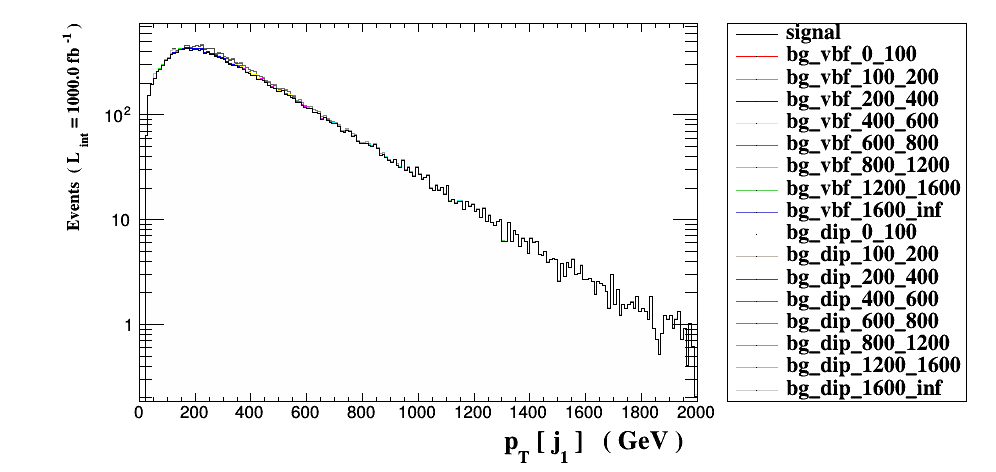
\includegraphics[scale=0.45]{selection_0.png}\\
\caption{   }
  \end{center}
\end{figure}
      \newpage
\subsection{ Histogram 2}

\textbf{* Plot: ETA ( jets[1] ) }\\
   \begin{table}[H]
  \begin{center}
    \begin{tabular}{|m{23.0mm}|m{23.0mm}|m{18.0mm}|m{19.0mm}|m{19.0mm}|m{19.0mm}|m{19.0mm}|}
      \hline
      {\cellcolor{yellow}         Dataset}& {\cellcolor{yellow}         Integral}& {\cellcolor{yellow}         Entries per event}& {\cellcolor{yellow}         Mean}& {\cellcolor{yellow}         RMS}& {\cellcolor{yellow}         \% underflow}& {\cellcolor{yellow}         \% overflow}\\
      \hline
      {\cellcolor{white}         signal}& {\cellcolor{white}         19174}& {\cellcolor{white}         1.0}& {\cellcolor{white}         -0.00426672}& {\cellcolor{white}         2.037}& {\cellcolor{green}         0.0}& {\cellcolor{green}         0.0}\\
      \hline
      {\cellcolor{white}         bg\_vbf\_0\_100}& {\cellcolor{white}         1.22}& {\cellcolor{white}         1.0}& {\cellcolor{white}         0.873486}& {\cellcolor{white}         2.934}& {\cellcolor{green}         0.0}& {\cellcolor{green}         0.0}\\
      \hline
      {\cellcolor{white}         bg\_vbf\_100\_200}& {\cellcolor{white}         29.1}& {\cellcolor{white}         1.0}& {\cellcolor{white}         0.133336}& {\cellcolor{white}         2.773}& {\cellcolor{green}         0.0}& {\cellcolor{green}         0.0}\\
      \hline
      {\cellcolor{white}         bg\_vbf\_200\_400}& {\cellcolor{white}         151}& {\cellcolor{white}         1.0}& {\cellcolor{white}         -0.006481}& {\cellcolor{white}         2.235}& {\cellcolor{green}         0.0}& {\cellcolor{green}         0.0}\\
      \hline
      {\cellcolor{white}         bg\_vbf\_400\_600}& {\cellcolor{white}         110}& {\cellcolor{white}         1.0}& {\cellcolor{white}         -0.0267496}& {\cellcolor{white}         1.928}& {\cellcolor{green}         0.0}& {\cellcolor{green}         0.0}\\
      \hline
      {\cellcolor{white}         bg\_vbf\_600\_800}& {\cellcolor{white}         41.0}& {\cellcolor{white}         1.0}& {\cellcolor{white}         0.00605067}& {\cellcolor{white}         1.754}& {\cellcolor{green}         0.0}& {\cellcolor{green}         0.0}\\
      \hline
      {\cellcolor{white}         bg\_vbf\_800\_1200}& {\cellcolor{white}         15.6}& {\cellcolor{white}         1.0}& {\cellcolor{white}         -0.0592612}& {\cellcolor{white}         1.598}& {\cellcolor{green}         0.0}& {\cellcolor{green}         0.0}\\
      \hline
      {\cellcolor{white}         bg\_vbf\_1200\_1600}& {\cellcolor{white}         1.37}& {\cellcolor{white}         1.0}& {\cellcolor{white}         -0.0746631}& {\cellcolor{white}         1.45}& {\cellcolor{green}         0.0}& {\cellcolor{green}         0.0}\\
      \hline
      {\cellcolor{white}         bg\_vbf\_1600\_inf}& {\cellcolor{white}         0.145}& {\cellcolor{white}         1.0}& {\cellcolor{white}         0.0871655}& {\cellcolor{white}         1.227}& {\cellcolor{green}         0.0}& {\cellcolor{green}         0.0}\\
      \hline
      {\cellcolor{white}         bg\_dip\_0\_100}& {\cellcolor{white}         0.0 +/\-- 0.0}& {\cellcolor{white}         0.}& {\cellcolor{white}         0.0}& {\cellcolor{white}         0.0}& {\cellcolor{green}         0.0}& {\cellcolor{green}         0.0}\\
      \hline
      {\cellcolor{white}         bg\_dip\_100\_200}& {\cellcolor{white}         79.0}& {\cellcolor{white}         1.0}& {\cellcolor{white}         1.65038}& {\cellcolor{white}         2.73}& {\cellcolor{green}         0.0}& {\cellcolor{green}         0.0}\\
      \hline
      {\cellcolor{white}         bg\_dip\_200\_400}& {\cellcolor{white}         477}& {\cellcolor{white}         1.0}& {\cellcolor{white}         0.146548}& {\cellcolor{white}         1.676}& {\cellcolor{green}         0.0}& {\cellcolor{green}         0.0}\\
      \hline
      {\cellcolor{white}         bg\_dip\_400\_600}& {\cellcolor{white}         306}& {\cellcolor{white}         1.0}& {\cellcolor{white}         0.1076}& {\cellcolor{white}         1.425}& {\cellcolor{green}         0.0}& {\cellcolor{green}         0.0}\\
      \hline
      {\cellcolor{white}         bg\_dip\_600\_800}& {\cellcolor{white}         90.0}& {\cellcolor{white}         1.0}& {\cellcolor{white}         -0.0364249}& {\cellcolor{white}         1.3}& {\cellcolor{green}         0.0}& {\cellcolor{green}         0.0}\\
      \hline
      {\cellcolor{white}         bg\_dip\_800\_1200}& {\cellcolor{white}         36.8}& {\cellcolor{white}         1.0}& {\cellcolor{white}         -0.0506134}& {\cellcolor{white}         1.215}& {\cellcolor{green}         0.0}& {\cellcolor{green}         0.0}\\
      \hline
      {\cellcolor{white}         bg\_dip\_1200\_1600}& {\cellcolor{white}         2.63}& {\cellcolor{white}         1.0}& {\cellcolor{white}         0.0264047}& {\cellcolor{white}         1.124}& {\cellcolor{green}         0.0}& {\cellcolor{green}         0.0}\\
      \hline
      {\cellcolor{white}         bg\_dip\_1600\_inf}& {\cellcolor{white}         0.244}& {\cellcolor{white}         1.0}& {\cellcolor{white}         -0.0490747}& {\cellcolor{white}         0.8389}& {\cellcolor{green}         0.0}& {\cellcolor{green}         0.0}\\
\hline
    \end{tabular}
  \end{center}
\end{table}

\begin{figure}[H]
  \begin{center}
    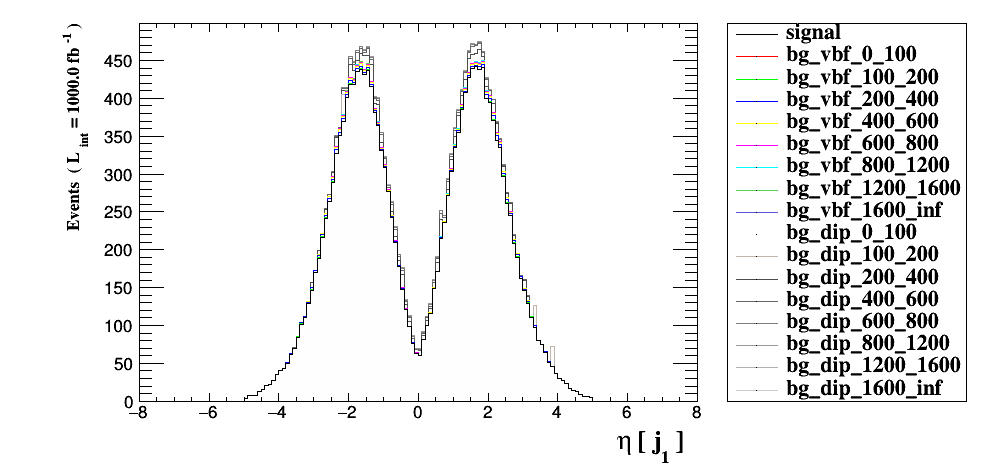
\includegraphics[scale=0.45]{selection_1.png}\\
\caption{   }
  \end{center}
\end{figure}
      \newpage
\subsection{ Histogram 3}

\textbf{* Plot: PHI ( jets[1] ) }\\
   \begin{table}[H]
  \begin{center}
    \begin{tabular}{|m{23.0mm}|m{23.0mm}|m{18.0mm}|m{19.0mm}|m{19.0mm}|m{19.0mm}|m{19.0mm}|}
      \hline
      {\cellcolor{yellow}         Dataset}& {\cellcolor{yellow}         Integral}& {\cellcolor{yellow}         Entries per event}& {\cellcolor{yellow}         Mean}& {\cellcolor{yellow}         RMS}& {\cellcolor{yellow}         \% underflow}& {\cellcolor{yellow}         \% overflow}\\
      \hline
      {\cellcolor{white}         signal}& {\cellcolor{white}         19174}& {\cellcolor{white}         1.0}& {\cellcolor{white}         0.00274665}& {\cellcolor{white}         1.814}& {\cellcolor{green}         0.0}& {\cellcolor{green}         0.0}\\
      \hline
      {\cellcolor{white}         bg\_vbf\_0\_100}& {\cellcolor{white}         1.22}& {\cellcolor{white}         1.0}& {\cellcolor{white}         -0.168141}& {\cellcolor{white}         1.997}& {\cellcolor{green}         0.0}& {\cellcolor{green}         0.0}\\
      \hline
      {\cellcolor{white}         bg\_vbf\_100\_200}& {\cellcolor{white}         29.1}& {\cellcolor{white}         1.0}& {\cellcolor{white}         -0.0767497}& {\cellcolor{white}         1.778}& {\cellcolor{green}         0.0}& {\cellcolor{green}         0.0}\\
      \hline
      {\cellcolor{white}         bg\_vbf\_200\_400}& {\cellcolor{white}         151}& {\cellcolor{white}         1.0}& {\cellcolor{white}         -0.0816388}& {\cellcolor{white}         1.818}& {\cellcolor{green}         0.0}& {\cellcolor{green}         0.0}\\
      \hline
      {\cellcolor{white}         bg\_vbf\_400\_600}& {\cellcolor{white}         110}& {\cellcolor{white}         1.0}& {\cellcolor{white}         0.0212645}& {\cellcolor{white}         1.801}& {\cellcolor{green}         0.0}& {\cellcolor{green}         0.0}\\
      \hline
      {\cellcolor{white}         bg\_vbf\_600\_800}& {\cellcolor{white}         41.0}& {\cellcolor{white}         1.0}& {\cellcolor{white}         -0.00569695}& {\cellcolor{white}         1.808}& {\cellcolor{green}         0.0}& {\cellcolor{green}         0.0}\\
      \hline
      {\cellcolor{white}         bg\_vbf\_800\_1200}& {\cellcolor{white}         15.6}& {\cellcolor{white}         1.0}& {\cellcolor{white}         0.0641089}& {\cellcolor{white}         1.814}& {\cellcolor{green}         0.0}& {\cellcolor{green}         0.0}\\
      \hline
      {\cellcolor{white}         bg\_vbf\_1200\_1600}& {\cellcolor{white}         1.37}& {\cellcolor{white}         1.0}& {\cellcolor{white}         0.0646329}& {\cellcolor{white}         1.787}& {\cellcolor{green}         0.0}& {\cellcolor{green}         0.0}\\
      \hline
      {\cellcolor{white}         bg\_vbf\_1600\_inf}& {\cellcolor{white}         0.145}& {\cellcolor{white}         1.0}& {\cellcolor{white}         0.217904}& {\cellcolor{white}         1.755}& {\cellcolor{green}         0.0}& {\cellcolor{green}         0.0}\\
      \hline
      {\cellcolor{white}         bg\_dip\_0\_100}& {\cellcolor{white}         0.0 +/\-- 0.0}& {\cellcolor{white}         0.}& {\cellcolor{white}         0.0}& {\cellcolor{white}         0.0}& {\cellcolor{green}         0.0}& {\cellcolor{green}         0.0}\\
      \hline
      {\cellcolor{white}         bg\_dip\_100\_200}& {\cellcolor{white}         79.0}& {\cellcolor{white}         1.0}& {\cellcolor{white}         0.466209}& {\cellcolor{white}         0.3607}& {\cellcolor{green}         0.0}& {\cellcolor{green}         0.0}\\
      \hline
      {\cellcolor{white}         bg\_dip\_200\_400}& {\cellcolor{white}         477}& {\cellcolor{white}         1.0}& {\cellcolor{white}         -0.0522949}& {\cellcolor{white}         1.826}& {\cellcolor{green}         0.0}& {\cellcolor{green}         0.0}\\
      \hline
      {\cellcolor{white}         bg\_dip\_400\_600}& {\cellcolor{white}         306}& {\cellcolor{white}         1.0}& {\cellcolor{white}         -0.125515}& {\cellcolor{white}         1.849}& {\cellcolor{green}         0.0}& {\cellcolor{green}         0.0}\\
      \hline
      {\cellcolor{white}         bg\_dip\_600\_800}& {\cellcolor{white}         90.0}& {\cellcolor{white}         1.0}& {\cellcolor{white}         -0.113698}& {\cellcolor{white}         1.83}& {\cellcolor{green}         0.0}& {\cellcolor{green}         0.0}\\
      \hline
      {\cellcolor{white}         bg\_dip\_800\_1200}& {\cellcolor{white}         36.8}& {\cellcolor{white}         1.0}& {\cellcolor{white}         0.0576669}& {\cellcolor{white}         1.795}& {\cellcolor{green}         0.0}& {\cellcolor{green}         0.0}\\
      \hline
      {\cellcolor{white}         bg\_dip\_1200\_1600}& {\cellcolor{white}         2.63}& {\cellcolor{white}         1.0}& {\cellcolor{white}         -0.152016}& {\cellcolor{white}         1.941}& {\cellcolor{green}         0.0}& {\cellcolor{green}         0.0}\\
      \hline
      {\cellcolor{white}         bg\_dip\_1600\_inf}& {\cellcolor{white}         0.244}& {\cellcolor{white}         1.0}& {\cellcolor{white}         -0.0323032}& {\cellcolor{white}         1.815}& {\cellcolor{green}         0.0}& {\cellcolor{green}         0.0}\\
\hline
    \end{tabular}
  \end{center}
\end{table}

\begin{figure}[H]
  \begin{center}
    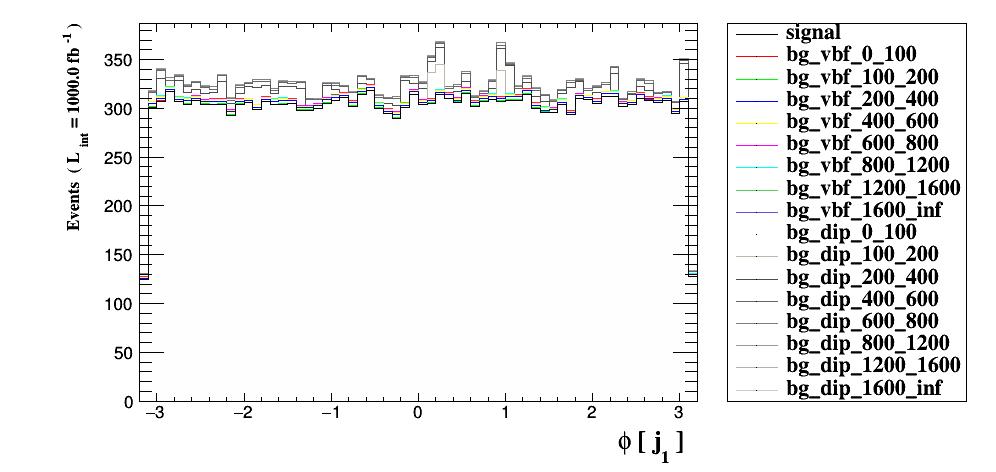
\includegraphics[scale=0.45]{selection_2.png}\\
\caption{   }
  \end{center}
\end{figure}
      \newpage
\subsection{ Histogram 4}

\textbf{* Plot: PT ( jets[2] ) }\\
   \begin{table}[H]
  \begin{center}
    \begin{tabular}{|m{23.0mm}|m{23.0mm}|m{18.0mm}|m{19.0mm}|m{19.0mm}|m{19.0mm}|m{19.0mm}|}
      \hline
      {\cellcolor{yellow}         Dataset}& {\cellcolor{yellow}         Integral}& {\cellcolor{yellow}         Entries per event}& {\cellcolor{yellow}         Mean}& {\cellcolor{yellow}         RMS}& {\cellcolor{yellow}         \% underflow}& {\cellcolor{yellow}         \% overflow}\\
      \hline
      {\cellcolor{white}         signal}& {\cellcolor{white}         19174}& {\cellcolor{white}         1.0}& {\cellcolor{white}         102.403}& {\cellcolor{white}         76.9}& {\cellcolor{green}         0.0}& {\cellcolor{green}         0.0}\\
      \hline
      {\cellcolor{white}         bg\_vbf\_0\_100}& {\cellcolor{white}         1.22}& {\cellcolor{white}         1.0}& {\cellcolor{white}         31.916}& {\cellcolor{white}         8.29}& {\cellcolor{green}         0.0}& {\cellcolor{green}         0.0}\\
      \hline
      {\cellcolor{white}         bg\_vbf\_100\_200}& {\cellcolor{white}         29.1}& {\cellcolor{white}         1.0}& {\cellcolor{white}         53.936}& {\cellcolor{white}         17.53}& {\cellcolor{green}         0.0}& {\cellcolor{green}         0.0}\\
      \hline
      {\cellcolor{white}         bg\_vbf\_200\_400}& {\cellcolor{white}         151}& {\cellcolor{white}         1.0}& {\cellcolor{white}         90.5854}& {\cellcolor{white}         37.67}& {\cellcolor{green}         0.0}& {\cellcolor{green}         0.0}\\
      \hline
      {\cellcolor{white}         bg\_vbf\_400\_600}& {\cellcolor{white}         110}& {\cellcolor{white}         1.0}& {\cellcolor{white}         125.017}& {\cellcolor{white}         60.47}& {\cellcolor{green}         0.0}& {\cellcolor{green}         0.0}\\
      \hline
      {\cellcolor{white}         bg\_vbf\_600\_800}& {\cellcolor{white}         41.0}& {\cellcolor{white}         1.0}& {\cellcolor{white}         168.787}& {\cellcolor{white}         85.77}& {\cellcolor{green}         0.0}& {\cellcolor{green}         0.0}\\
      \hline
      {\cellcolor{white}         bg\_vbf\_800\_1200}& {\cellcolor{white}         15.6}& {\cellcolor{white}         1.0}& {\cellcolor{white}         215.936}& {\cellcolor{white}         127.0}& {\cellcolor{green}         0.0}& {\cellcolor{green}         0.0}\\
      \hline
      {\cellcolor{white}         bg\_vbf\_1200\_1600}& {\cellcolor{white}         1.37}& {\cellcolor{white}         1.0}& {\cellcolor{white}         286.77}& {\cellcolor{white}         196.2}& {\cellcolor{green}         0.0}& {\cellcolor{green}         0.0}\\
      \hline
      {\cellcolor{white}         bg\_vbf\_1600\_inf}& {\cellcolor{white}         0.145}& {\cellcolor{white}         1.0}& {\cellcolor{white}         301.151}& {\cellcolor{white}         261.1}& {\cellcolor{green}         0.0}& {\cellcolor{green}         0.0}\\
      \hline
      {\cellcolor{white}         bg\_dip\_0\_100}& {\cellcolor{white}         0.0 +/\-- 0.0}& {\cellcolor{white}         0.}& {\cellcolor{white}         0.0}& {\cellcolor{white}         0.0}& {\cellcolor{green}         0.0}& {\cellcolor{green}         0.0}\\
      \hline
      {\cellcolor{white}         bg\_dip\_100\_200}& {\cellcolor{white}         79.0}& {\cellcolor{white}         1.0}& {\cellcolor{white}         49.3379}& {\cellcolor{white}         16.83}& {\cellcolor{green}         0.0}& {\cellcolor{green}         0.0}\\
      \hline
      {\cellcolor{white}         bg\_dip\_200\_400}& {\cellcolor{white}         477}& {\cellcolor{white}         1.0}& {\cellcolor{white}         68.617}& {\cellcolor{white}         36.13}& {\cellcolor{green}         0.0}& {\cellcolor{green}         0.0}\\
      \hline
      {\cellcolor{white}         bg\_dip\_400\_600}& {\cellcolor{white}         306}& {\cellcolor{white}         1.0}& {\cellcolor{white}         78.6224}& {\cellcolor{white}         56.28}& {\cellcolor{green}         0.0}& {\cellcolor{green}         0.0}\\
      \hline
      {\cellcolor{white}         bg\_dip\_600\_800}& {\cellcolor{white}         90.0}& {\cellcolor{white}         1.0}& {\cellcolor{white}         94.6258}& {\cellcolor{white}         83.07}& {\cellcolor{green}         0.0}& {\cellcolor{green}         0.0}\\
      \hline
      {\cellcolor{white}         bg\_dip\_800\_1200}& {\cellcolor{white}         36.8}& {\cellcolor{white}         1.0}& {\cellcolor{white}         124.553}& {\cellcolor{white}         124.0}& {\cellcolor{green}         0.0}& {\cellcolor{green}         0.0}\\
      \hline
      {\cellcolor{white}         bg\_dip\_1200\_1600}& {\cellcolor{white}         2.63}& {\cellcolor{white}         1.0}& {\cellcolor{white}         176.706}& {\cellcolor{white}         198.4}& {\cellcolor{green}         0.0}& {\cellcolor{green}         0.0}\\
      \hline
      {\cellcolor{white}         bg\_dip\_1600\_inf}& {\cellcolor{white}         0.244}& {\cellcolor{white}         1.0}& {\cellcolor{white}         138.5}& {\cellcolor{white}         204.7}& {\cellcolor{green}         0.0}& {\cellcolor{green}         0.0}\\
\hline
    \end{tabular}
  \end{center}
\end{table}

\begin{figure}[H]
  \begin{center}
    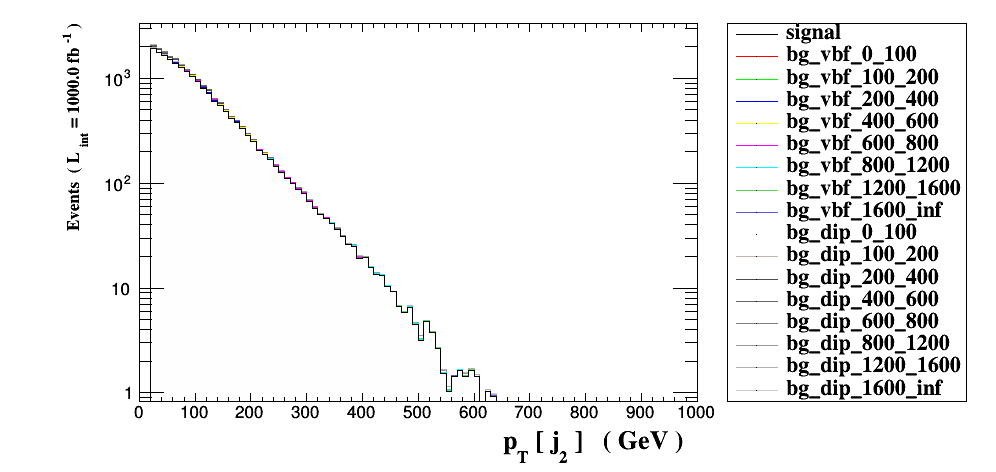
\includegraphics[scale=0.45]{selection_3.png}\\
\caption{   }
  \end{center}
\end{figure}
      \newpage
\subsection{ Histogram 5}

\textbf{* Plot: ETA ( jets[2] ) }\\
   \begin{table}[H]
  \begin{center}
    \begin{tabular}{|m{23.0mm}|m{23.0mm}|m{18.0mm}|m{19.0mm}|m{19.0mm}|m{19.0mm}|m{19.0mm}|}
      \hline
      {\cellcolor{yellow}         Dataset}& {\cellcolor{yellow}         Integral}& {\cellcolor{yellow}         Entries per event}& {\cellcolor{yellow}         Mean}& {\cellcolor{yellow}         RMS}& {\cellcolor{yellow}         \% underflow}& {\cellcolor{yellow}         \% overflow}\\
      \hline
      {\cellcolor{white}         signal}& {\cellcolor{white}         19174}& {\cellcolor{white}         1.0}& {\cellcolor{white}         0.00824761}& {\cellcolor{white}         3.058}& {\cellcolor{green}         0.0}& {\cellcolor{green}         0.0}\\
      \hline
      {\cellcolor{white}         bg\_vbf\_0\_100}& {\cellcolor{white}         1.22}& {\cellcolor{white}         1.0}& {\cellcolor{white}         1.04772}& {\cellcolor{white}         3.507}& {\cellcolor{green}         0.0}& {\cellcolor{green}         0.0}\\
      \hline
      {\cellcolor{white}         bg\_vbf\_100\_200}& {\cellcolor{white}         29.1}& {\cellcolor{white}         1.0}& {\cellcolor{white}         -0.324417}& {\cellcolor{white}         3.174}& {\cellcolor{green}         0.0}& {\cellcolor{green}         0.0}\\
      \hline
      {\cellcolor{white}         bg\_vbf\_200\_400}& {\cellcolor{white}         151}& {\cellcolor{white}         1.0}& {\cellcolor{white}         0.0275519}& {\cellcolor{white}         2.946}& {\cellcolor{green}         0.0}& {\cellcolor{green}         0.0}\\
      \hline
      {\cellcolor{white}         bg\_vbf\_400\_600}& {\cellcolor{white}         110}& {\cellcolor{white}         1.0}& {\cellcolor{white}         0.0664249}& {\cellcolor{white}         2.847}& {\cellcolor{green}         0.0}& {\cellcolor{green}         0.0}\\
      \hline
      {\cellcolor{white}         bg\_vbf\_600\_800}& {\cellcolor{white}         41.0}& {\cellcolor{white}         1.0}& {\cellcolor{white}         -0.00657983}& {\cellcolor{white}         2.765}& {\cellcolor{green}         0.0}& {\cellcolor{green}         0.0}\\
      \hline
      {\cellcolor{white}         bg\_vbf\_800\_1200}& {\cellcolor{white}         15.6}& {\cellcolor{white}         1.0}& {\cellcolor{white}         0.123933}& {\cellcolor{white}         2.754}& {\cellcolor{green}         0.0}& {\cellcolor{green}         0.0}\\
      \hline
      {\cellcolor{white}         bg\_vbf\_1200\_1600}& {\cellcolor{white}         1.37}& {\cellcolor{white}         1.0}& {\cellcolor{white}         0.151477}& {\cellcolor{white}         2.787}& {\cellcolor{green}         0.0}& {\cellcolor{green}         0.0}\\
      \hline
      {\cellcolor{white}         bg\_vbf\_1600\_inf}& {\cellcolor{white}         0.145}& {\cellcolor{white}         1.0}& {\cellcolor{white}         -0.203626}& {\cellcolor{white}         2.95}& {\cellcolor{green}         0.0}& {\cellcolor{green}         0.0}\\
      \hline
      {\cellcolor{white}         bg\_dip\_0\_100}& {\cellcolor{white}         0.0 +/\-- 0.0}& {\cellcolor{white}         0.}& {\cellcolor{white}         0.0}& {\cellcolor{white}         0.0}& {\cellcolor{green}         0.0}& {\cellcolor{green}         0.0}\\
      \hline
      {\cellcolor{white}         bg\_dip\_100\_200}& {\cellcolor{white}         79.0}& {\cellcolor{white}         1.0}& {\cellcolor{white}         0.140052}& {\cellcolor{white}         2.918}& {\cellcolor{green}         0.0}& {\cellcolor{green}         0.0}\\
      \hline
      {\cellcolor{white}         bg\_dip\_200\_400}& {\cellcolor{white}         477}& {\cellcolor{white}         1.0}& {\cellcolor{white}         0.291332}& {\cellcolor{white}         3.134}& {\cellcolor{green}         0.0}& {\cellcolor{green}         0.0}\\
      \hline
      {\cellcolor{white}         bg\_dip\_400\_600}& {\cellcolor{white}         306}& {\cellcolor{white}         1.0}& {\cellcolor{white}         -0.0693841}& {\cellcolor{white}         3.116}& {\cellcolor{green}         0.0}& {\cellcolor{green}         0.0}\\
      \hline
      {\cellcolor{white}         bg\_dip\_600\_800}& {\cellcolor{white}         90.0}& {\cellcolor{white}         1.0}& {\cellcolor{white}         0.0792687}& {\cellcolor{white}         3.236}& {\cellcolor{green}         0.0}& {\cellcolor{green}         0.0}\\
      \hline
      {\cellcolor{white}         bg\_dip\_800\_1200}& {\cellcolor{white}         36.8}& {\cellcolor{white}         1.0}& {\cellcolor{white}         0.0158785}& {\cellcolor{white}         3.221}& {\cellcolor{green}         0.0}& {\cellcolor{green}         0.0}\\
      \hline
      {\cellcolor{white}         bg\_dip\_1200\_1600}& {\cellcolor{white}         2.63}& {\cellcolor{white}         1.0}& {\cellcolor{white}         -0.142349}& {\cellcolor{white}         3.23}& {\cellcolor{green}         0.0}& {\cellcolor{green}         0.0}\\
      \hline
      {\cellcolor{white}         bg\_dip\_1600\_inf}& {\cellcolor{white}         0.244}& {\cellcolor{white}         1.0}& {\cellcolor{white}         -0.328753}& {\cellcolor{white}         3.419}& {\cellcolor{green}         0.0}& {\cellcolor{green}         0.0}\\
\hline
    \end{tabular}
  \end{center}
\end{table}

\begin{figure}[H]
  \begin{center}
    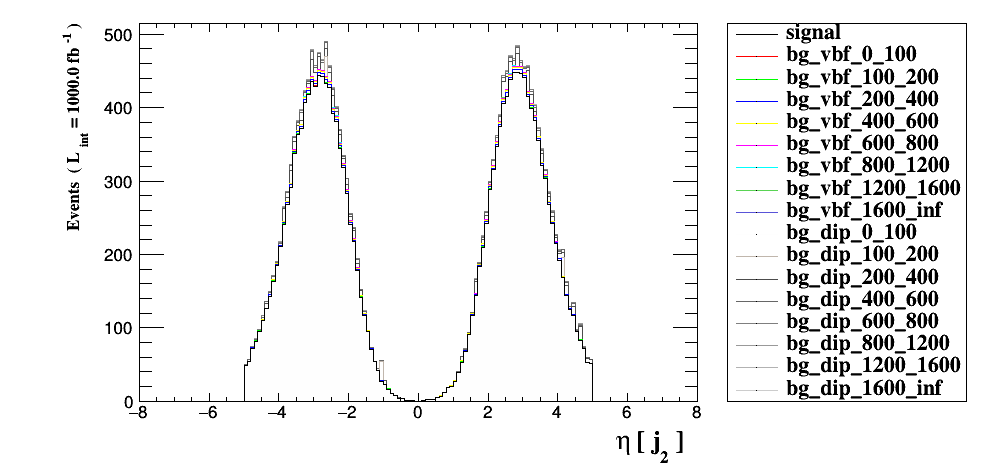
\includegraphics[scale=0.45]{selection_4.png}\\
\caption{   }
  \end{center}
\end{figure}
      \newpage
\subsection{ Histogram 6}

\textbf{* Plot: PHI ( jets[2] ) }\\
   \begin{table}[H]
  \begin{center}
    \begin{tabular}{|m{23.0mm}|m{23.0mm}|m{18.0mm}|m{19.0mm}|m{19.0mm}|m{19.0mm}|m{19.0mm}|}
      \hline
      {\cellcolor{yellow}         Dataset}& {\cellcolor{yellow}         Integral}& {\cellcolor{yellow}         Entries per event}& {\cellcolor{yellow}         Mean}& {\cellcolor{yellow}         RMS}& {\cellcolor{yellow}         \% underflow}& {\cellcolor{yellow}         \% overflow}\\
      \hline
      {\cellcolor{white}         signal}& {\cellcolor{white}         19174}& {\cellcolor{white}         1.0}& {\cellcolor{white}         -0.00468976}& {\cellcolor{white}         1.813}& {\cellcolor{green}         0.0}& {\cellcolor{green}         0.0}\\
      \hline
      {\cellcolor{white}         bg\_vbf\_0\_100}& {\cellcolor{white}         1.22}& {\cellcolor{white}         1.0}& {\cellcolor{white}         0.0859607}& {\cellcolor{white}         1.498}& {\cellcolor{green}         0.0}& {\cellcolor{green}         0.0}\\
      \hline
      {\cellcolor{white}         bg\_vbf\_100\_200}& {\cellcolor{white}         29.1}& {\cellcolor{white}         1.0}& {\cellcolor{white}         0.17327}& {\cellcolor{white}         1.879}& {\cellcolor{green}         0.0}& {\cellcolor{green}         0.0}\\
      \hline
      {\cellcolor{white}         bg\_vbf\_200\_400}& {\cellcolor{white}         151}& {\cellcolor{white}         1.0}& {\cellcolor{white}         -0.0817648}& {\cellcolor{white}         1.828}& {\cellcolor{green}         0.0}& {\cellcolor{green}         0.0}\\
      \hline
      {\cellcolor{white}         bg\_vbf\_400\_600}& {\cellcolor{white}         110}& {\cellcolor{white}         1.0}& {\cellcolor{white}         -0.0599984}& {\cellcolor{white}         1.828}& {\cellcolor{green}         0.0}& {\cellcolor{green}         0.0}\\
      \hline
      {\cellcolor{white}         bg\_vbf\_600\_800}& {\cellcolor{white}         41.0}& {\cellcolor{white}         1.0}& {\cellcolor{white}         0.0117494}& {\cellcolor{white}         1.812}& {\cellcolor{green}         0.0}& {\cellcolor{green}         0.0}\\
      \hline
      {\cellcolor{white}         bg\_vbf\_800\_1200}& {\cellcolor{white}         15.6}& {\cellcolor{white}         1.0}& {\cellcolor{white}         -0.0684445}& {\cellcolor{white}         1.824}& {\cellcolor{green}         0.0}& {\cellcolor{green}         0.0}\\
      \hline
      {\cellcolor{white}         bg\_vbf\_1200\_1600}& {\cellcolor{white}         1.37}& {\cellcolor{white}         1.0}& {\cellcolor{white}         -0.0586342}& {\cellcolor{white}         1.806}& {\cellcolor{green}         0.0}& {\cellcolor{green}         0.0}\\
      \hline
      {\cellcolor{white}         bg\_vbf\_1600\_inf}& {\cellcolor{white}         0.145}& {\cellcolor{white}         1.0}& {\cellcolor{white}         -0.198205}& {\cellcolor{white}         1.858}& {\cellcolor{green}         0.0}& {\cellcolor{green}         0.0}\\
      \hline
      {\cellcolor{white}         bg\_dip\_0\_100}& {\cellcolor{white}         0.0 +/\-- 0.0}& {\cellcolor{white}         0.}& {\cellcolor{white}         0.0}& {\cellcolor{white}         0.0}& {\cellcolor{green}         0.0}& {\cellcolor{green}         0.0}\\
      \hline
      {\cellcolor{white}         bg\_dip\_100\_200}& {\cellcolor{white}         79.0}& {\cellcolor{white}         1.0}& {\cellcolor{white}         1.00733}& {\cellcolor{white}         1.634}& {\cellcolor{green}         0.0}& {\cellcolor{green}         0.0}\\
      \hline
      {\cellcolor{white}         bg\_dip\_200\_400}& {\cellcolor{white}         477}& {\cellcolor{white}         1.0}& {\cellcolor{white}         -0.0248154}& {\cellcolor{white}         1.887}& {\cellcolor{green}         0.0}& {\cellcolor{green}         0.0}\\
      \hline
      {\cellcolor{white}         bg\_dip\_400\_600}& {\cellcolor{white}         306}& {\cellcolor{white}         1.0}& {\cellcolor{white}         -0.0373808}& {\cellcolor{white}         1.79}& {\cellcolor{green}         0.0}& {\cellcolor{green}         0.0}\\
      \hline
      {\cellcolor{white}         bg\_dip\_600\_800}& {\cellcolor{white}         90.0}& {\cellcolor{white}         1.0}& {\cellcolor{white}         0.0797356}& {\cellcolor{white}         1.824}& {\cellcolor{green}         0.0}& {\cellcolor{green}         0.0}\\
      \hline
      {\cellcolor{white}         bg\_dip\_800\_1200}& {\cellcolor{white}         36.8}& {\cellcolor{white}         1.0}& {\cellcolor{white}         0.124598}& {\cellcolor{white}         1.781}& {\cellcolor{green}         0.0}& {\cellcolor{green}         0.0}\\
      \hline
      {\cellcolor{white}         bg\_dip\_1200\_1600}& {\cellcolor{white}         2.63}& {\cellcolor{white}         1.0}& {\cellcolor{white}         -0.323666}& {\cellcolor{white}         1.753}& {\cellcolor{green}         0.0}& {\cellcolor{green}         0.0}\\
      \hline
      {\cellcolor{white}         bg\_dip\_1600\_inf}& {\cellcolor{white}         0.244}& {\cellcolor{white}         1.0}& {\cellcolor{white}         -0.421228}& {\cellcolor{white}         1.806}& {\cellcolor{green}         0.0}& {\cellcolor{green}         0.0}\\
\hline
    \end{tabular}
  \end{center}
\end{table}

\begin{figure}[H]
  \begin{center}
    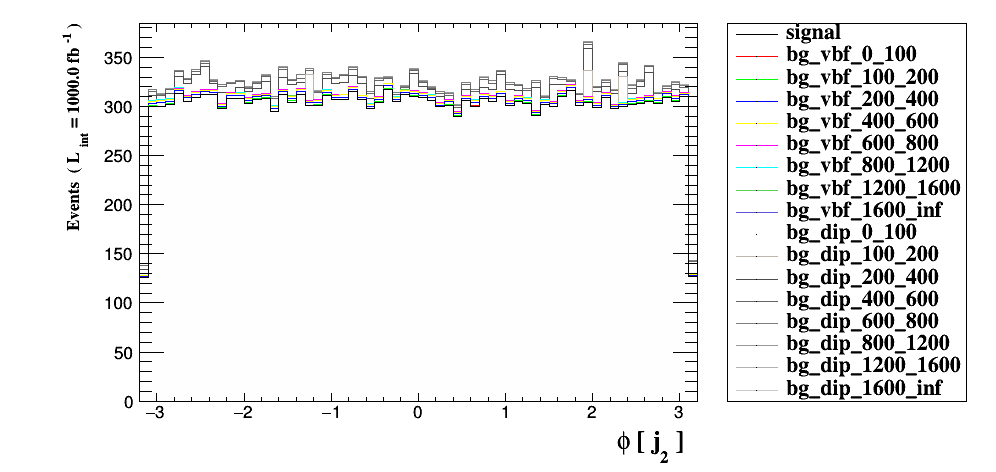
\includegraphics[scale=0.45]{selection_5.png}\\
\caption{   }
  \end{center}
\end{figure}
      \newpage
\subsection{ Histogram 7}

\textbf{* Plot: DELTAR ( jets[1] , jets[2] ) }\\
   \begin{table}[H]
  \begin{center}
    \begin{tabular}{|m{23.0mm}|m{23.0mm}|m{18.0mm}|m{19.0mm}|m{19.0mm}|m{19.0mm}|m{19.0mm}|}
      \hline
      {\cellcolor{yellow}         Dataset}& {\cellcolor{yellow}         Integral}& {\cellcolor{yellow}         Entries per event}& {\cellcolor{yellow}         Mean}& {\cellcolor{yellow}         RMS}& {\cellcolor{yellow}         \% underflow}& {\cellcolor{yellow}         \% overflow}\\
      \hline
      {\cellcolor{white}         signal}& {\cellcolor{white}         19174}& {\cellcolor{white}         1.0}& {\cellcolor{white}         5.1046}& {\cellcolor{white}         1.028}& {\cellcolor{green}         0.0}& {\cellcolor{green}         0.0}\\
      \hline
      {\cellcolor{white}         bg\_vbf\_0\_100}& {\cellcolor{white}         1.22}& {\cellcolor{white}         1.0}& {\cellcolor{white}         6.62263}& {\cellcolor{white}         0.3293}& {\cellcolor{green}         0.0}& {\cellcolor{green}         0.0}\\
      \hline
      {\cellcolor{white}         bg\_vbf\_100\_200}& {\cellcolor{white}         29.1}& {\cellcolor{white}         1.0}& {\cellcolor{white}         5.99091}& {\cellcolor{white}         0.8146}& {\cellcolor{green}         0.0}& {\cellcolor{green}         0.0}\\
      \hline
      {\cellcolor{white}         bg\_vbf\_200\_400}& {\cellcolor{white}         151}& {\cellcolor{white}         1.0}& {\cellcolor{white}         5.24335}& {\cellcolor{white}         0.8413}& {\cellcolor{green}         0.0}& {\cellcolor{green}         0.0}\\
      \hline
      {\cellcolor{white}         bg\_vbf\_400\_600}& {\cellcolor{white}         110}& {\cellcolor{white}         1.0}& {\cellcolor{white}         4.96829}& {\cellcolor{white}         0.7025}& {\cellcolor{green}         0.0}& {\cellcolor{green}         0.0}\\
      \hline
      {\cellcolor{white}         bg\_vbf\_600\_800}& {\cellcolor{white}         41.0}& {\cellcolor{white}         1.0}& {\cellcolor{white}         4.83273}& {\cellcolor{white}         0.5935}& {\cellcolor{green}         0.0}& {\cellcolor{green}         0.0}\\
      \hline
      {\cellcolor{white}         bg\_vbf\_800\_1200}& {\cellcolor{white}         15.6}& {\cellcolor{white}         1.0}& {\cellcolor{white}         4.73982}& {\cellcolor{white}         0.5158}& {\cellcolor{green}         0.0}& {\cellcolor{green}         0.0}\\
      \hline
      {\cellcolor{white}         bg\_vbf\_1200\_1600}& {\cellcolor{white}         1.37}& {\cellcolor{white}         1.0}& {\cellcolor{white}         4.67427}& {\cellcolor{white}         0.4511}& {\cellcolor{green}         0.0}& {\cellcolor{green}         0.0}\\
      \hline
      {\cellcolor{white}         bg\_vbf\_1600\_inf}& {\cellcolor{white}         0.145}& {\cellcolor{white}         1.0}& {\cellcolor{white}         4.62399}& {\cellcolor{white}         0.461}& {\cellcolor{green}         0.0}& {\cellcolor{green}         0.0}\\
      \hline
      {\cellcolor{white}         bg\_dip\_0\_100}& {\cellcolor{white}         0.0 +/\-- 0.0}& {\cellcolor{white}         0.}& {\cellcolor{white}         0.0}& {\cellcolor{white}         0.0}& {\cellcolor{green}         0.0}& {\cellcolor{green}         0.0}\\
      \hline
      {\cellcolor{white}         bg\_dip\_100\_200}& {\cellcolor{white}         79.0}& {\cellcolor{white}         1.0}& {\cellcolor{white}         5.99929}& {\cellcolor{white}         0.4811}& {\cellcolor{green}         0.0}& {\cellcolor{green}         0.0}\\
      \hline
      {\cellcolor{white}         bg\_dip\_200\_400}& {\cellcolor{white}         477}& {\cellcolor{white}         1.0}& {\cellcolor{white}         4.87458}& {\cellcolor{white}         0.6286}& {\cellcolor{green}         0.0}& {\cellcolor{green}         0.0}\\
      \hline
      {\cellcolor{white}         bg\_dip\_400\_600}& {\cellcolor{white}         306}& {\cellcolor{white}         1.0}& {\cellcolor{white}         4.6746}& {\cellcolor{white}         0.5749}& {\cellcolor{green}         0.0}& {\cellcolor{green}         0.0}\\
      \hline
      {\cellcolor{white}         bg\_dip\_600\_800}& {\cellcolor{white}         90.0}& {\cellcolor{white}         1.0}& {\cellcolor{white}         4.64892}& {\cellcolor{white}         0.5595}& {\cellcolor{green}         0.0}& {\cellcolor{green}         0.0}\\
      \hline
      {\cellcolor{white}         bg\_dip\_800\_1200}& {\cellcolor{white}         36.8}& {\cellcolor{white}         1.0}& {\cellcolor{white}         4.61435}& {\cellcolor{white}         0.495}& {\cellcolor{green}         0.0}& {\cellcolor{green}         0.0}\\
      \hline
      {\cellcolor{white}         bg\_dip\_1200\_1600}& {\cellcolor{white}         2.63}& {\cellcolor{white}         1.0}& {\cellcolor{white}         4.51401}& {\cellcolor{white}         0.442}& {\cellcolor{green}         0.0}& {\cellcolor{green}         0.0}\\
      \hline
      {\cellcolor{white}         bg\_dip\_1600\_inf}& {\cellcolor{white}         0.244}& {\cellcolor{white}         1.0}& {\cellcolor{white}         4.44387}& {\cellcolor{white}         0.4353}& {\cellcolor{green}         0.0}& {\cellcolor{green}         0.0}\\
\hline
    \end{tabular}
  \end{center}
\end{table}

\begin{figure}[H]
  \begin{center}
    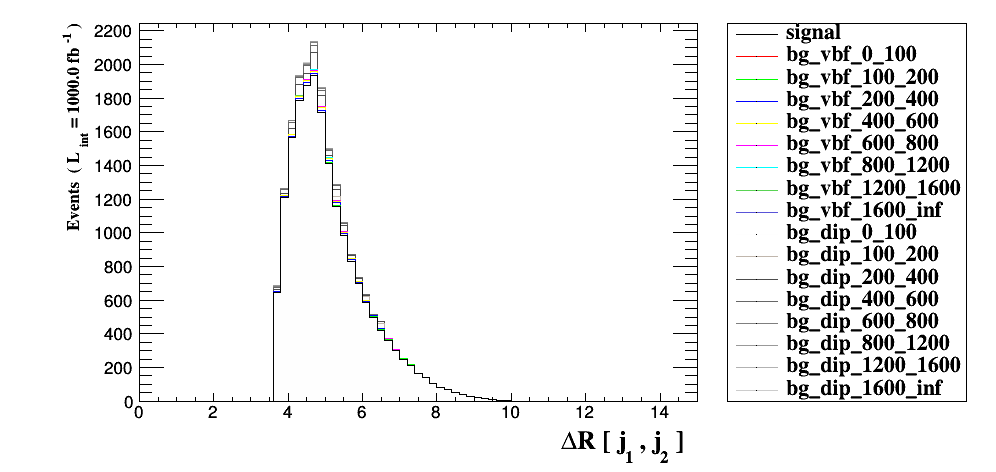
\includegraphics[scale=0.45]{selection_6.png}\\
\caption{   }
  \end{center}
\end{figure}
      \newpage
\subsection{ Histogram 8}

\textbf{* Plot: M ( jets[1] jets[2] ) }\\
   \begin{table}[H]
  \begin{center}
    \begin{tabular}{|m{23.0mm}|m{23.0mm}|m{18.0mm}|m{19.0mm}|m{19.0mm}|m{19.0mm}|m{19.0mm}|}
      \hline
      {\cellcolor{yellow}         Dataset}& {\cellcolor{yellow}         Integral}& {\cellcolor{yellow}         Entries per event}& {\cellcolor{yellow}         Mean}& {\cellcolor{yellow}         RMS}& {\cellcolor{yellow}         \% underflow}& {\cellcolor{yellow}         \% overflow}\\
      \hline
      {\cellcolor{white}         signal}& {\cellcolor{white}         19174}& {\cellcolor{white}         1.0}& {\cellcolor{white}         1797.17}& {\cellcolor{white}         804.0}& {\cellcolor{green}         0.0}& {\cellcolor{green}         0.0}\\
      \hline
      {\cellcolor{white}         bg\_vbf\_0\_100}& {\cellcolor{white}         1.22}& {\cellcolor{white}         1.0}& {\cellcolor{white}         886.102}& {\cellcolor{white}         84.95}& {\cellcolor{green}         0.0}& {\cellcolor{green}         0.0}\\
      \hline
      {\cellcolor{white}         bg\_vbf\_100\_200}& {\cellcolor{white}         29.1}& {\cellcolor{white}         1.0}& {\cellcolor{white}         1373.99}& {\cellcolor{white}         562.4}& {\cellcolor{green}         0.0}& {\cellcolor{green}         0.0}\\
      \hline
      {\cellcolor{white}         bg\_vbf\_200\_400}& {\cellcolor{white}         151}& {\cellcolor{white}         1.0}& {\cellcolor{white}         1686.56}& {\cellcolor{white}         787.6}& {\cellcolor{green}         0.0}& {\cellcolor{green}         0.0}\\
      \hline
      {\cellcolor{white}         bg\_vbf\_400\_600}& {\cellcolor{white}         110}& {\cellcolor{white}         1.0}& {\cellcolor{white}         2066.12}& {\cellcolor{white}         824.9}& {\cellcolor{green}         0.0}& {\cellcolor{green}         0.0}\\
      \hline
      {\cellcolor{white}         bg\_vbf\_600\_800}& {\cellcolor{white}         41.0}& {\cellcolor{white}         1.0}& {\cellcolor{white}         2497.1}& {\cellcolor{white}         840.0}& {\cellcolor{green}         0.0}& {\cellcolor{green}         0.0}\\
      \hline
      {\cellcolor{white}         bg\_vbf\_800\_1200}& {\cellcolor{white}         15.6}& {\cellcolor{white}         1.0}& {\cellcolor{white}         2990.13}& {\cellcolor{white}         928.2}& {\cellcolor{green}         0.0}& {\cellcolor{green}         0.0}\\
      \hline
      {\cellcolor{white}         bg\_vbf\_1200\_1600}& {\cellcolor{white}         1.37}& {\cellcolor{white}         1.0}& {\cellcolor{white}         3719.45}& {\cellcolor{white}         1119}& {\cellcolor{green}         0.0}& {\cellcolor{green}         0.03938}\\
      \hline
      {\cellcolor{white}         bg\_vbf\_1600\_inf}& {\cellcolor{white}         0.145}& {\cellcolor{white}         1.0}& {\cellcolor{white}         4126.54}& {\cellcolor{white}         1410}& {\cellcolor{green}         0.0}& {\cellcolor{green}         0.4886}\\
      \hline
      {\cellcolor{white}         bg\_dip\_0\_100}& {\cellcolor{white}         0.0 +/\-- 0.0}& {\cellcolor{white}         0.}& {\cellcolor{white}         0.0}& {\cellcolor{white}         0.0}& {\cellcolor{green}         0.0}& {\cellcolor{green}         0.0}\\
      \hline
      {\cellcolor{white}         bg\_dip\_100\_200}& {\cellcolor{white}         79.0}& {\cellcolor{white}         1.0}& {\cellcolor{white}         1172.68}& {\cellcolor{white}         166.8}& {\cellcolor{green}         0.0}& {\cellcolor{green}         0.0}\\
      \hline
      {\cellcolor{white}         bg\_dip\_200\_400}& {\cellcolor{white}         477}& {\cellcolor{white}         1.0}& {\cellcolor{white}         1168.01}& {\cellcolor{white}         358.4}& {\cellcolor{green}         0.0}& {\cellcolor{green}         0.0}\\
      \hline
      {\cellcolor{white}         bg\_dip\_400\_600}& {\cellcolor{white}         306}& {\cellcolor{white}         1.0}& {\cellcolor{white}         1373.0}& {\cellcolor{white}         458.4}& {\cellcolor{green}         0.0}& {\cellcolor{green}         0.0}\\
      \hline
      {\cellcolor{white}         bg\_dip\_600\_800}& {\cellcolor{white}         90.0}& {\cellcolor{white}         1.0}& {\cellcolor{white}         1704.65}& {\cellcolor{white}         623.1}& {\cellcolor{green}         0.0}& {\cellcolor{green}         0.0}\\
      \hline
      {\cellcolor{white}         bg\_dip\_800\_1200}& {\cellcolor{white}         36.8}& {\cellcolor{white}         1.0}& {\cellcolor{white}         2097.6}& {\cellcolor{white}         885.2}& {\cellcolor{green}         0.0}& {\cellcolor{green}         0.0}\\
      \hline
      {\cellcolor{white}         bg\_dip\_1200\_1600}& {\cellcolor{white}         2.63}& {\cellcolor{white}         1.0}& {\cellcolor{white}         2709.62}& {\cellcolor{white}         1239}& {\cellcolor{green}         0.0}& {\cellcolor{green}         0.0}\\
      \hline
      {\cellcolor{white}         bg\_dip\_1600\_inf}& {\cellcolor{white}         0.244}& {\cellcolor{white}         1.0}& {\cellcolor{white}         2721.5}& {\cellcolor{white}         1274}& {\cellcolor{green}         0.0}& {\cellcolor{green}         0.0}\\
\hline
    \end{tabular}
  \end{center}
\end{table}

\begin{figure}[H]
  \begin{center}
    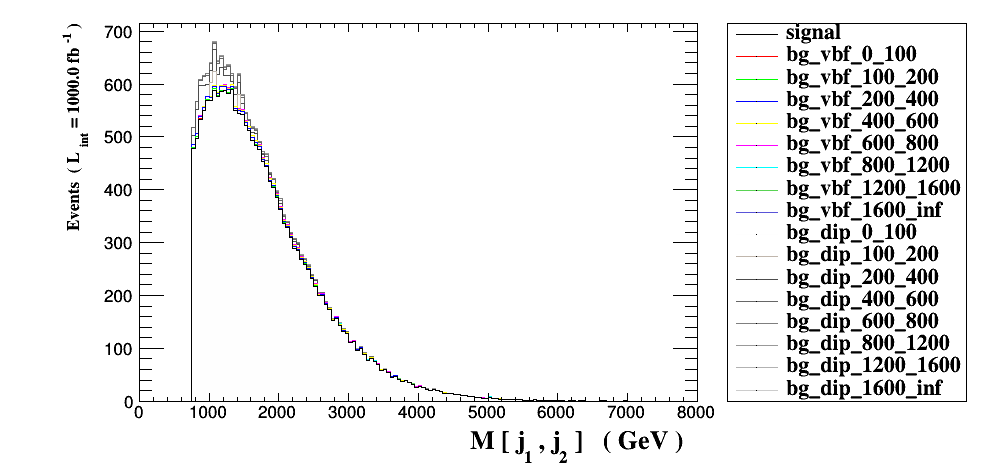
\includegraphics[scale=0.45]{selection_7.png}\\
\caption{   }
  \end{center}
\end{figure}
      \newpage
\subsection{ Histogram 9}

\textbf{* Plot: MET}\\
   \begin{table}[H]
  \begin{center}
    \begin{tabular}{|m{23.0mm}|m{23.0mm}|m{18.0mm}|m{19.0mm}|m{19.0mm}|m{19.0mm}|m{19.0mm}|}
      \hline
      {\cellcolor{yellow}         Dataset}& {\cellcolor{yellow}         Integral}& {\cellcolor{yellow}         Entries per event}& {\cellcolor{yellow}         Mean}& {\cellcolor{yellow}         RMS}& {\cellcolor{yellow}         \% underflow}& {\cellcolor{yellow}         \% overflow}\\
      \hline
      {\cellcolor{white}         signal}& {\cellcolor{white}         19174}& {\cellcolor{white}         1.0}& {\cellcolor{white}         9.23621e-09}& {\cellcolor{white}         1.193e-08}& {\cellcolor{green}         0.0}& {\cellcolor{green}         0.0}\\
      \hline
      {\cellcolor{white}         bg\_vbf\_0\_100}& {\cellcolor{white}         1.22}& {\cellcolor{white}         1.0}& {\cellcolor{white}         2.92664e-09}& {\cellcolor{white}         2.061e-09}& {\cellcolor{green}         0.0}& {\cellcolor{green}         0.0}\\
      \hline
      {\cellcolor{white}         bg\_vbf\_100\_200}& {\cellcolor{white}         29.1}& {\cellcolor{white}         1.0}& {\cellcolor{white}         4.59216e-09}& {\cellcolor{white}         2.634e-09}& {\cellcolor{green}         0.0}& {\cellcolor{green}         0.0}\\
      \hline
      {\cellcolor{white}         bg\_vbf\_200\_400}& {\cellcolor{white}         151}& {\cellcolor{white}         1.0}& {\cellcolor{white}         5.28184e-09}& {\cellcolor{white}         3.059e-09}& {\cellcolor{green}         0.0}& {\cellcolor{green}         0.0}\\
      \hline
      {\cellcolor{white}         bg\_vbf\_400\_600}& {\cellcolor{white}         110}& {\cellcolor{white}         1.0}& {\cellcolor{white}         5.56314e-09}& {\cellcolor{white}         3.759e-09}& {\cellcolor{green}         0.0}& {\cellcolor{green}         0.0}\\
      \hline
      {\cellcolor{white}         bg\_vbf\_600\_800}& {\cellcolor{white}         41.0}& {\cellcolor{white}         1.0}& {\cellcolor{white}         5.7028e-09}& {\cellcolor{white}         3.425e-09}& {\cellcolor{green}         0.0}& {\cellcolor{green}         0.0}\\
      \hline
      {\cellcolor{white}         bg\_vbf\_800\_1200}& {\cellcolor{white}         15.6}& {\cellcolor{white}         1.0}& {\cellcolor{white}         6.73764e-09}& {\cellcolor{white}         5.92e-09}& {\cellcolor{green}         0.0}& {\cellcolor{green}         0.0}\\
      \hline
      {\cellcolor{white}         bg\_vbf\_1200\_1600}& {\cellcolor{white}         1.37}& {\cellcolor{white}         1.0}& {\cellcolor{white}         1.72505e-08}& {\cellcolor{white}         1.831e-08}& {\cellcolor{green}         0.0}& {\cellcolor{green}         0.0}\\
      \hline
      {\cellcolor{white}         bg\_vbf\_1600\_inf}& {\cellcolor{white}         0.145}& {\cellcolor{white}         1.0}& {\cellcolor{white}         3.09154e-08}& {\cellcolor{white}         2.364e-08}& {\cellcolor{green}         0.0}& {\cellcolor{green}         0.0}\\
      \hline
      {\cellcolor{white}         bg\_dip\_0\_100}& {\cellcolor{white}         0.0 +/\-- 0.0}& {\cellcolor{white}         0.}& {\cellcolor{white}         0.0}& {\cellcolor{white}         0.0}& {\cellcolor{green}         0.0}& {\cellcolor{green}         0.0}\\
      \hline
      {\cellcolor{white}         bg\_dip\_100\_200}& {\cellcolor{white}         79.0}& {\cellcolor{white}         1.0}& {\cellcolor{white}         2.6048e-09}& {\cellcolor{white}         5.584e-10}& {\cellcolor{green}         0.0}& {\cellcolor{green}         0.0}\\
      \hline
      {\cellcolor{white}         bg\_dip\_200\_400}& {\cellcolor{white}         477}& {\cellcolor{white}         1.0}& {\cellcolor{white}         5.15652e-09}& {\cellcolor{white}         2.886e-09}& {\cellcolor{green}         0.0}& {\cellcolor{green}         0.0}\\
      \hline
      {\cellcolor{white}         bg\_dip\_400\_600}& {\cellcolor{white}         306}& {\cellcolor{white}         1.0}& {\cellcolor{white}         5.26293e-09}& {\cellcolor{white}         2.848e-09}& {\cellcolor{green}         0.0}& {\cellcolor{green}         0.0}\\
      \hline
      {\cellcolor{white}         bg\_dip\_600\_800}& {\cellcolor{white}         90.0}& {\cellcolor{white}         1.0}& {\cellcolor{white}         5.42862e-09}& {\cellcolor{white}         2.905e-09}& {\cellcolor{green}         0.0}& {\cellcolor{green}         0.0}\\
      \hline
      {\cellcolor{white}         bg\_dip\_800\_1200}& {\cellcolor{white}         36.8}& {\cellcolor{white}         1.0}& {\cellcolor{white}         7.13192e-09}& {\cellcolor{white}         8.331e-09}& {\cellcolor{green}         0.0}& {\cellcolor{green}         0.0}\\
      \hline
      {\cellcolor{white}         bg\_dip\_1200\_1600}& {\cellcolor{white}         2.63}& {\cellcolor{white}         1.0}& {\cellcolor{white}         2.55869e-08}& {\cellcolor{white}         2.401e-08}& {\cellcolor{green}         0.0}& {\cellcolor{green}         0.0}\\
      \hline
      {\cellcolor{white}         bg\_dip\_1600\_inf}& {\cellcolor{white}         0.244}& {\cellcolor{white}         1.0}& {\cellcolor{white}         3.47198e-08}& {\cellcolor{white}         2.306e-08}& {\cellcolor{green}         0.0}& {\cellcolor{green}         0.0}\\
\hline
    \end{tabular}
  \end{center}
\end{table}

\begin{figure}[H]
  \begin{center}
    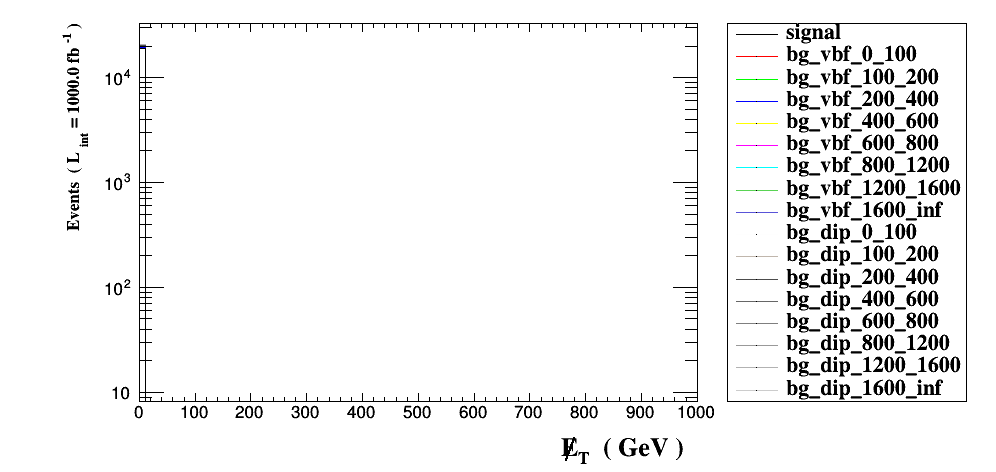
\includegraphics[scale=0.45]{selection_8.png}\\
\caption{   }
  \end{center}
\end{figure}
      \newpage
\subsection{ Histogram 10}

\textbf{* Plot: sdETA ( jets[1] jets[2] ) }\\
   \begin{table}[H]
  \begin{center}
    \begin{tabular}{|m{23.0mm}|m{23.0mm}|m{18.0mm}|m{19.0mm}|m{19.0mm}|m{19.0mm}|m{19.0mm}|}
      \hline
      {\cellcolor{yellow}         Dataset}& {\cellcolor{yellow}         Integral}& {\cellcolor{yellow}         Entries per event}& {\cellcolor{yellow}         Mean}& {\cellcolor{yellow}         RMS}& {\cellcolor{yellow}         \% underflow}& {\cellcolor{yellow}         \% overflow}\\
      \hline
      {\cellcolor{white}         signal}& {\cellcolor{white}         19174}& {\cellcolor{white}         1.0}& {\cellcolor{white}         -0.0125143}& {\cellcolor{white}         4.892}& {\cellcolor{green}         0.0}& {\cellcolor{green}         0.0}\\
      \hline
      {\cellcolor{white}         bg\_vbf\_0\_100}& {\cellcolor{white}         1.22}& {\cellcolor{white}         1.0}& {\cellcolor{white}         -0.174236}& {\cellcolor{white}         6.403}& {\cellcolor{green}         0.0}& {\cellcolor{green}         0.0}\\
      \hline
      {\cellcolor{white}         bg\_vbf\_100\_200}& {\cellcolor{white}         29.1}& {\cellcolor{white}         1.0}& {\cellcolor{white}         0.457753}& {\cellcolor{white}         5.752}& {\cellcolor{green}         0.0}& {\cellcolor{green}         0.0}\\
      \hline
      {\cellcolor{white}         bg\_vbf\_200\_400}& {\cellcolor{white}         151}& {\cellcolor{white}         1.0}& {\cellcolor{white}         -0.0340329}& {\cellcolor{white}         5.008}& {\cellcolor{green}         0.0}& {\cellcolor{green}         0.0}\\
      \hline
      {\cellcolor{white}         bg\_vbf\_400\_600}& {\cellcolor{white}         110}& {\cellcolor{white}         1.0}& {\cellcolor{white}         -0.0931745}& {\cellcolor{white}         4.618}& {\cellcolor{green}         0.0}& {\cellcolor{green}         0.0}\\
      \hline
      {\cellcolor{white}         bg\_vbf\_600\_800}& {\cellcolor{white}         41.0}& {\cellcolor{white}         1.0}& {\cellcolor{white}         0.0126305}& {\cellcolor{white}         4.376}& {\cellcolor{green}         0.0}& {\cellcolor{green}         0.0}\\
      \hline
      {\cellcolor{white}         bg\_vbf\_800\_1200}& {\cellcolor{white}         15.6}& {\cellcolor{white}         1.0}& {\cellcolor{white}         -0.183195}& {\cellcolor{white}         4.209}& {\cellcolor{green}         0.0}& {\cellcolor{green}         0.0}\\
      \hline
      {\cellcolor{white}         bg\_vbf\_1200\_1600}& {\cellcolor{white}         1.37}& {\cellcolor{white}         1.0}& {\cellcolor{white}         -0.226141}& {\cellcolor{white}         4.078}& {\cellcolor{green}         0.0}& {\cellcolor{green}         0.0}\\
      \hline
      {\cellcolor{white}         bg\_vbf\_1600\_inf}& {\cellcolor{white}         0.145}& {\cellcolor{white}         1.0}& {\cellcolor{white}         0.290791}& {\cellcolor{white}         3.996}& {\cellcolor{green}         0.0}& {\cellcolor{green}         0.0}\\
      \hline
      {\cellcolor{white}         bg\_dip\_0\_100}& {\cellcolor{white}         0.0 +/\-- 0.0}& {\cellcolor{white}         0.}& {\cellcolor{white}         0.0}& {\cellcolor{white}         0.0}& {\cellcolor{green}         0.0}& {\cellcolor{green}         0.0}\\
      \hline
      {\cellcolor{white}         bg\_dip\_100\_200}& {\cellcolor{white}         79.0}& {\cellcolor{white}         1.0}& {\cellcolor{white}         1.51032}& {\cellcolor{white}         5.585}& {\cellcolor{green}         0.0}& {\cellcolor{green}         0.0}\\
      \hline
      {\cellcolor{white}         bg\_dip\_200\_400}& {\cellcolor{white}         477}& {\cellcolor{white}         1.0}& {\cellcolor{white}         -0.144784}& {\cellcolor{white}         4.518}& {\cellcolor{green}         0.0}& {\cellcolor{green}         0.0}\\
      \hline
      {\cellcolor{white}         bg\_dip\_400\_600}& {\cellcolor{white}         306}& {\cellcolor{white}         1.0}& {\cellcolor{white}         0.176984}& {\cellcolor{white}         4.26}& {\cellcolor{green}         0.0}& {\cellcolor{green}         0.0}\\
      \hline
      {\cellcolor{white}         bg\_dip\_600\_800}& {\cellcolor{white}         90.0}& {\cellcolor{white}         1.0}& {\cellcolor{white}         -0.115694}& {\cellcolor{white}         4.219}& {\cellcolor{green}         0.0}& {\cellcolor{green}         0.0}\\
      \hline
      {\cellcolor{white}         bg\_dip\_800\_1200}& {\cellcolor{white}         36.8}& {\cellcolor{white}         1.0}& {\cellcolor{white}         -0.0664918}& {\cellcolor{white}         4.119}& {\cellcolor{green}         0.0}& {\cellcolor{green}         0.0}\\
      \hline
      {\cellcolor{white}         bg\_dip\_1200\_1600}& {\cellcolor{white}         2.63}& {\cellcolor{white}         1.0}& {\cellcolor{white}         0.168753}& {\cellcolor{white}         4.051}& {\cellcolor{green}         0.0}& {\cellcolor{green}         0.0}\\
      \hline
      {\cellcolor{white}         bg\_dip\_1600\_inf}& {\cellcolor{white}         0.244}& {\cellcolor{white}         1.0}& {\cellcolor{white}         0.279678}& {\cellcolor{white}         4.007}& {\cellcolor{green}         0.0}& {\cellcolor{green}         0.0}\\
\hline
    \end{tabular}
  \end{center}
\end{table}

\begin{figure}[H]
  \begin{center}
    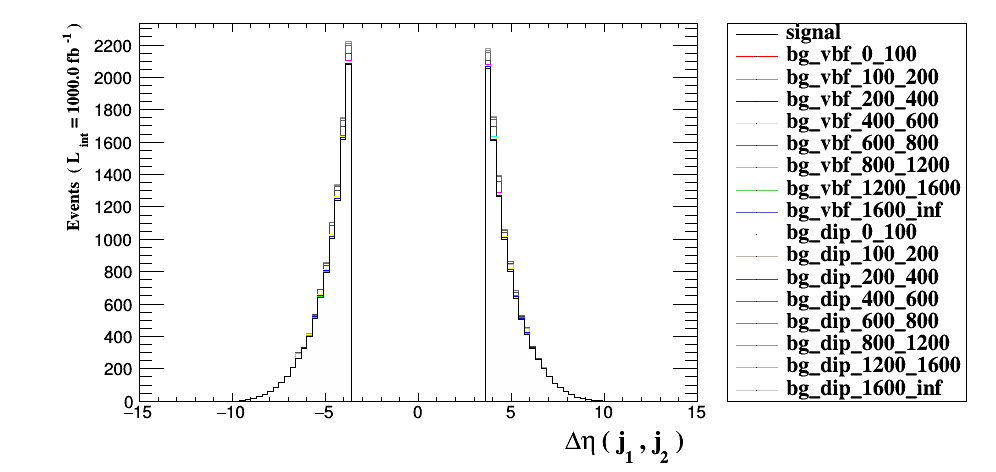
\includegraphics[scale=0.45]{selection_9.png}\\
\caption{   }
  \end{center}
\end{figure}
      \newpage
\subsection{ Histogram 11}

\textbf{* Plot: M ( a[1] a[2] ) }\\
   \begin{table}[H]
  \begin{center}
    \begin{tabular}{|m{23.0mm}|m{23.0mm}|m{18.0mm}|m{19.0mm}|m{19.0mm}|m{19.0mm}|m{19.0mm}|}
      \hline
      {\cellcolor{yellow}         Dataset}& {\cellcolor{yellow}         Integral}& {\cellcolor{yellow}         Entries per event}& {\cellcolor{yellow}         Mean}& {\cellcolor{yellow}         RMS}& {\cellcolor{yellow}         \% underflow}& {\cellcolor{yellow}         \% overflow}\\
      \hline
      {\cellcolor{white}         signal}& {\cellcolor{white}         19174}& {\cellcolor{white}         1.0}& {\cellcolor{white}         1364.91}& {\cellcolor{white}         757.5}& {\cellcolor{green}         0.0}& {\cellcolor{green}         0.9384}\\
      \hline
      {\cellcolor{white}         bg\_vbf\_0\_100}& {\cellcolor{white}         1.22}& {\cellcolor{white}         1.0}& {\cellcolor{white}         999.408}& {\cellcolor{white}         375.3}& {\cellcolor{green}         0.0}& {\cellcolor{green}         0.0}\\
      \hline
      {\cellcolor{white}         bg\_vbf\_100\_200}& {\cellcolor{white}         29.1}& {\cellcolor{white}         1.0}& {\cellcolor{white}         847.835}& {\cellcolor{white}         279.9}& {\cellcolor{green}         0.0}& {\cellcolor{green}         0.0}\\
      \hline
      {\cellcolor{white}         bg\_vbf\_200\_400}& {\cellcolor{white}         151}& {\cellcolor{white}         1.0}& {\cellcolor{white}         806.306}& {\cellcolor{white}         333.7}& {\cellcolor{green}         0.0}& {\cellcolor{green}         0.0}\\
      \hline
      {\cellcolor{white}         bg\_vbf\_400\_600}& {\cellcolor{white}         110}& {\cellcolor{white}         1.0}& {\cellcolor{white}         757.771}& {\cellcolor{white}         293.6}& {\cellcolor{green}         0.0}& {\cellcolor{green}         0.0}\\
      \hline
      {\cellcolor{white}         bg\_vbf\_600\_800}& {\cellcolor{white}         41.0}& {\cellcolor{white}         1.0}& {\cellcolor{white}         774.989}& {\cellcolor{white}         292.6}& {\cellcolor{green}         0.0}& {\cellcolor{green}         0.0}\\
      \hline
      {\cellcolor{white}         bg\_vbf\_800\_1200}& {\cellcolor{white}         15.6}& {\cellcolor{white}         1.0}& {\cellcolor{white}         795.097}& {\cellcolor{white}         304.5}& {\cellcolor{green}         0.0}& {\cellcolor{green}         0.0}\\
      \hline
      {\cellcolor{white}         bg\_vbf\_1200\_1600}& {\cellcolor{white}         1.37}& {\cellcolor{white}         1.0}& {\cellcolor{white}         827.522}& {\cellcolor{white}         348.5}& {\cellcolor{green}         0.0}& {\cellcolor{green}         0.0}\\
      \hline
      {\cellcolor{white}         bg\_vbf\_1600\_inf}& {\cellcolor{white}         0.145}& {\cellcolor{white}         1.0}& {\cellcolor{white}         902.86}& {\cellcolor{white}         410.2}& {\cellcolor{green}         0.0}& {\cellcolor{green}         0.0}\\
      \hline
      {\cellcolor{white}         bg\_dip\_0\_100}& {\cellcolor{white}         0.0 +/\-- 0.0}& {\cellcolor{white}         0.}& {\cellcolor{white}         0.0}& {\cellcolor{white}         0.0}& {\cellcolor{green}         0.0}& {\cellcolor{green}         0.0}\\
      \hline
      {\cellcolor{white}         bg\_dip\_100\_200}& {\cellcolor{white}         79.0}& {\cellcolor{white}         1.0}& {\cellcolor{white}         674.287}& {\cellcolor{white}         36.08}& {\cellcolor{green}         0.0}& {\cellcolor{green}         0.0}\\
      \hline
      {\cellcolor{white}         bg\_dip\_200\_400}& {\cellcolor{white}         477}& {\cellcolor{white}         1.0}& {\cellcolor{white}         785.534}& {\cellcolor{white}         368.8}& {\cellcolor{green}         0.0}& {\cellcolor{green}         0.0}\\
      \hline
      {\cellcolor{white}         bg\_dip\_400\_600}& {\cellcolor{white}         306}& {\cellcolor{white}         1.0}& {\cellcolor{white}         771.771}& {\cellcolor{white}         325.2}& {\cellcolor{green}         0.0}& {\cellcolor{green}         0.0}\\
      \hline
      {\cellcolor{white}         bg\_dip\_600\_800}& {\cellcolor{white}         90.0}& {\cellcolor{white}         1.0}& {\cellcolor{white}         805.657}& {\cellcolor{white}         366.8}& {\cellcolor{green}         0.0}& {\cellcolor{green}         0.0}\\
      \hline
      {\cellcolor{white}         bg\_dip\_800\_1200}& {\cellcolor{white}         36.8}& {\cellcolor{white}         1.0}& {\cellcolor{white}         805.114}& {\cellcolor{white}         335.3}& {\cellcolor{green}         0.0}& {\cellcolor{green}         0.0}\\
      \hline
      {\cellcolor{white}         bg\_dip\_1200\_1600}& {\cellcolor{white}         2.63}& {\cellcolor{white}         1.0}& {\cellcolor{white}         924.629}& {\cellcolor{white}         435.1}& {\cellcolor{green}         0.0}& {\cellcolor{green}         0.0}\\
      \hline
      {\cellcolor{white}         bg\_dip\_1600\_inf}& {\cellcolor{white}         0.244}& {\cellcolor{white}         1.0}& {\cellcolor{white}         930.522}& {\cellcolor{white}         452.3}& {\cellcolor{green}         0.0}& {\cellcolor{green}         0.0}\\
\hline
    \end{tabular}
  \end{center}
\end{table}

\begin{figure}[H]
  \begin{center}
    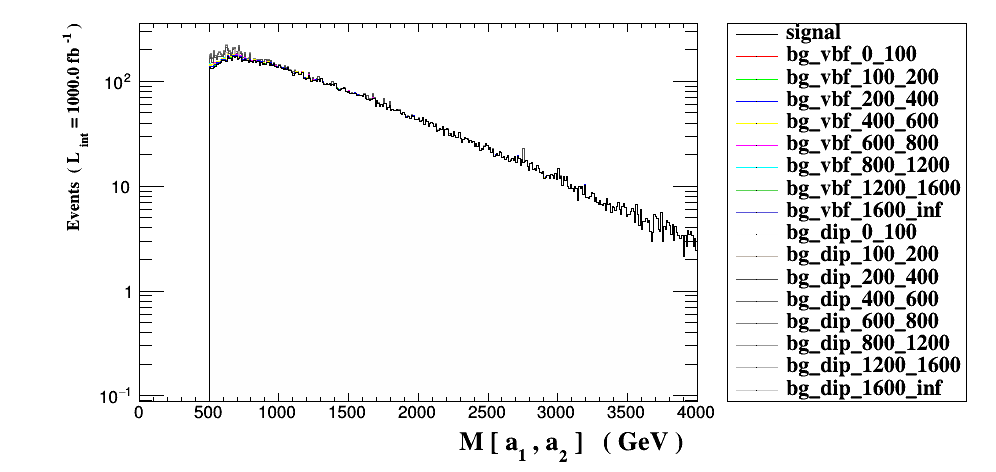
\includegraphics[scale=0.45]{selection_10.png}\\
\caption{   }
  \end{center}
\end{figure}
      \newpage
\subsection{ Histogram 12}

\textbf{* Plot: PT ( a[1] ) }\\
   \begin{table}[H]
  \begin{center}
    \begin{tabular}{|m{23.0mm}|m{23.0mm}|m{18.0mm}|m{19.0mm}|m{19.0mm}|m{19.0mm}|m{19.0mm}|}
      \hline
      {\cellcolor{yellow}         Dataset}& {\cellcolor{yellow}         Integral}& {\cellcolor{yellow}         Entries per event}& {\cellcolor{yellow}         Mean}& {\cellcolor{yellow}         RMS}& {\cellcolor{yellow}         \% underflow}& {\cellcolor{yellow}         \% overflow}\\
      \hline
      {\cellcolor{white}         signal}& {\cellcolor{white}         19174}& {\cellcolor{white}         1.0}& {\cellcolor{white}         718.918}& {\cellcolor{white}         350.1}& {\cellcolor{green}         0.0}& {\cellcolor{green}         0.7195}\\
      \hline
      {\cellcolor{white}         bg\_vbf\_0\_100}& {\cellcolor{white}         1.22}& {\cellcolor{white}         1.0}& {\cellcolor{white}         379.899}& {\cellcolor{white}         64.59}& {\cellcolor{green}         0.0}& {\cellcolor{green}         0.0}\\
      \hline
      {\cellcolor{white}         bg\_vbf\_100\_200}& {\cellcolor{white}         29.1}& {\cellcolor{white}         1.0}& {\cellcolor{white}         373.902}& {\cellcolor{white}         77.67}& {\cellcolor{green}         0.0}& {\cellcolor{green}         0.0}\\
      \hline
      {\cellcolor{white}         bg\_vbf\_200\_400}& {\cellcolor{white}         151}& {\cellcolor{white}         1.0}& {\cellcolor{white}         391.46}& {\cellcolor{white}         92.25}& {\cellcolor{green}         0.0}& {\cellcolor{green}         0.0}\\
      \hline
      {\cellcolor{white}         bg\_vbf\_400\_600}& {\cellcolor{white}         110}& {\cellcolor{white}         1.0}& {\cellcolor{white}         436.107}& {\cellcolor{white}         113.9}& {\cellcolor{green}         0.0}& {\cellcolor{green}         0.0}\\
      \hline
      {\cellcolor{white}         bg\_vbf\_600\_800}& {\cellcolor{white}         41.0}& {\cellcolor{white}         1.0}& {\cellcolor{white}         516.8}& {\cellcolor{white}         150.3}& {\cellcolor{green}         0.0}& {\cellcolor{green}         0.0}\\
      \hline
      {\cellcolor{white}         bg\_vbf\_800\_1200}& {\cellcolor{white}         15.6}& {\cellcolor{white}         1.0}& {\cellcolor{white}         657.311}& {\cellcolor{white}         223.5}& {\cellcolor{green}         0.0}& {\cellcolor{green}         0.0}\\
      \hline
      {\cellcolor{white}         bg\_vbf\_1200\_1600}& {\cellcolor{white}         1.37}& {\cellcolor{white}         1.0}& {\cellcolor{white}         890.939}& {\cellcolor{white}         358.6}& {\cellcolor{green}         0.0}& {\cellcolor{green}         0.07854}\\
      \hline
      {\cellcolor{white}         bg\_vbf\_1600\_inf}& {\cellcolor{white}         0.145}& {\cellcolor{white}         1.0}& {\cellcolor{white}         1323.7}& {\cellcolor{white}         534.5}& {\cellcolor{orange}         0.0}& {\cellcolor{orange}         6.344}\\
      \hline
      {\cellcolor{white}         bg\_dip\_0\_100}& {\cellcolor{white}         0.0 +/\-- 0.0}& {\cellcolor{white}         0.}& {\cellcolor{white}         0.0}& {\cellcolor{white}         0.0}& {\cellcolor{green}         0.0}& {\cellcolor{green}         0.0}\\
      \hline
      {\cellcolor{white}         bg\_dip\_100\_200}& {\cellcolor{white}         79.0}& {\cellcolor{white}         1.0}& {\cellcolor{white}         327.174}& {\cellcolor{white}         7.434}& {\cellcolor{green}         0.0}& {\cellcolor{green}         0.0}\\
      \hline
      {\cellcolor{white}         bg\_dip\_200\_400}& {\cellcolor{white}         477}& {\cellcolor{white}         1.0}& {\cellcolor{white}         393.477}& {\cellcolor{white}         77.89}& {\cellcolor{green}         0.0}& {\cellcolor{green}         0.0}\\
      \hline
      {\cellcolor{white}         bg\_dip\_400\_600}& {\cellcolor{white}         306}& {\cellcolor{white}         1.0}& {\cellcolor{white}         475.422}& {\cellcolor{white}         123.4}& {\cellcolor{green}         0.0}& {\cellcolor{green}         0.0}\\
      \hline
      {\cellcolor{white}         bg\_dip\_600\_800}& {\cellcolor{white}         90.0}& {\cellcolor{white}         1.0}& {\cellcolor{white}         603.382}& {\cellcolor{white}         164.2}& {\cellcolor{green}         0.0}& {\cellcolor{green}         0.0}\\
      \hline
      {\cellcolor{white}         bg\_dip\_800\_1200}& {\cellcolor{white}         36.8}& {\cellcolor{white}         1.0}& {\cellcolor{white}         778.016}& {\cellcolor{white}         241.8}& {\cellcolor{green}         0.0}& {\cellcolor{green}         0.0}\\
      \hline
      {\cellcolor{white}         bg\_dip\_1200\_1600}& {\cellcolor{white}         2.63}& {\cellcolor{white}         1.0}& {\cellcolor{white}         1095.08}& {\cellcolor{white}         412.4}& {\cellcolor{green}         0.0}& {\cellcolor{green}         0.0}\\
      \hline
      {\cellcolor{white}         bg\_dip\_1600\_inf}& {\cellcolor{white}         0.244}& {\cellcolor{white}         1.0}& {\cellcolor{white}         1602.75}& {\cellcolor{white}         495.3}& {\cellcolor{red}         0.0}& {\cellcolor{red}         18.53}\\
\hline
    \end{tabular}
  \end{center}
\end{table}

\begin{figure}[H]
  \begin{center}
    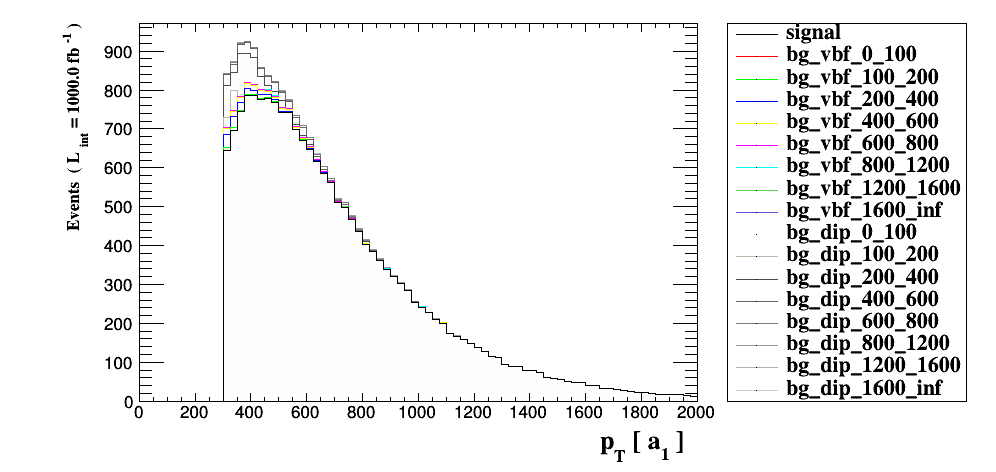
\includegraphics[scale=0.45]{selection_11.png}\\
\caption{   }
  \end{center}
\end{figure}
      \newpage
\subsection{ Histogram 13}

\textbf{* Plot: PT ( a[2] ) }\\
   \begin{table}[H]
  \begin{center}
    \begin{tabular}{|m{23.0mm}|m{23.0mm}|m{18.0mm}|m{19.0mm}|m{19.0mm}|m{19.0mm}|m{19.0mm}|}
      \hline
      {\cellcolor{yellow}         Dataset}& {\cellcolor{yellow}         Integral}& {\cellcolor{yellow}         Entries per event}& {\cellcolor{yellow}         Mean}& {\cellcolor{yellow}         RMS}& {\cellcolor{yellow}         \% underflow}& {\cellcolor{yellow}         \% overflow}\\
      \hline
      {\cellcolor{white}         signal}& {\cellcolor{white}         19174}& {\cellcolor{white}         1.0}& {\cellcolor{white}         486.902}& {\cellcolor{white}         328.9}& {\cellcolor{green}         0.0}& {\cellcolor{green}         0.3176}\\
      \hline
      {\cellcolor{white}         bg\_vbf\_0\_100}& {\cellcolor{white}         1.22}& {\cellcolor{white}         1.0}& {\cellcolor{white}         359.837}& {\cellcolor{white}         74.21}& {\cellcolor{green}         0.0}& {\cellcolor{green}         0.0}\\
      \hline
      {\cellcolor{white}         bg\_vbf\_100\_200}& {\cellcolor{white}         29.1}& {\cellcolor{white}         1.0}& {\cellcolor{white}         285.217}& {\cellcolor{white}         94.57}& {\cellcolor{green}         0.0}& {\cellcolor{green}         0.0}\\
      \hline
      {\cellcolor{white}         bg\_vbf\_200\_400}& {\cellcolor{white}         151}& {\cellcolor{white}         1.0}& {\cellcolor{white}         209.251}& {\cellcolor{white}         118.9}& {\cellcolor{green}         0.0}& {\cellcolor{green}         0.0}\\
      \hline
      {\cellcolor{white}         bg\_vbf\_400\_600}& {\cellcolor{white}         110}& {\cellcolor{white}         1.0}& {\cellcolor{white}         159.332}& {\cellcolor{white}         118.8}& {\cellcolor{green}         0.0}& {\cellcolor{green}         0.0}\\
      \hline
      {\cellcolor{white}         bg\_vbf\_600\_800}& {\cellcolor{white}         41.0}& {\cellcolor{white}         1.0}& {\cellcolor{white}         157.378}& {\cellcolor{white}         113.0}& {\cellcolor{green}         0.0}& {\cellcolor{green}         0.0}\\
      \hline
      {\cellcolor{white}         bg\_vbf\_800\_1200}& {\cellcolor{white}         15.6}& {\cellcolor{white}         1.0}& {\cellcolor{white}         159.508}& {\cellcolor{white}         121.4}& {\cellcolor{green}         0.0}& {\cellcolor{green}         0.0}\\
      \hline
      {\cellcolor{white}         bg\_vbf\_1200\_1600}& {\cellcolor{white}         1.37}& {\cellcolor{white}         1.0}& {\cellcolor{white}         167.561}& {\cellcolor{white}         142.6}& {\cellcolor{green}         0.0}& {\cellcolor{green}         0.0}\\
      \hline
      {\cellcolor{white}         bg\_vbf\_1600\_inf}& {\cellcolor{white}         0.145}& {\cellcolor{white}         1.0}& {\cellcolor{white}         183.782}& {\cellcolor{white}         190.2}& {\cellcolor{green}         0.0}& {\cellcolor{green}         0.0}\\
      \hline
      {\cellcolor{white}         bg\_dip\_0\_100}& {\cellcolor{white}         0.0 +/\-- 0.0}& {\cellcolor{white}         0.}& {\cellcolor{white}         0.0}& {\cellcolor{white}         0.0}& {\cellcolor{green}         0.0}& {\cellcolor{green}         0.0}\\
      \hline
      {\cellcolor{white}         bg\_dip\_100\_200}& {\cellcolor{white}         79.0}& {\cellcolor{white}         1.0}& {\cellcolor{white}         253.391}& {\cellcolor{white}         44.39}& {\cellcolor{green}         0.0}& {\cellcolor{green}         0.0}\\
      \hline
      {\cellcolor{white}         bg\_dip\_200\_400}& {\cellcolor{white}         477}& {\cellcolor{white}         1.0}& {\cellcolor{white}         186.1}& {\cellcolor{white}         97.8}& {\cellcolor{green}         0.0}& {\cellcolor{green}         0.0}\\
      \hline
      {\cellcolor{white}         bg\_dip\_400\_600}& {\cellcolor{white}         306}& {\cellcolor{white}         1.0}& {\cellcolor{white}         144.408}& {\cellcolor{white}         100.8}& {\cellcolor{green}         0.0}& {\cellcolor{green}         0.0}\\
      \hline
      {\cellcolor{white}         bg\_dip\_600\_800}& {\cellcolor{white}         90.0}& {\cellcolor{white}         1.0}& {\cellcolor{white}         140.303}& {\cellcolor{white}         115.8}& {\cellcolor{green}         0.0}& {\cellcolor{green}         0.0}\\
      \hline
      {\cellcolor{white}         bg\_dip\_800\_1200}& {\cellcolor{white}         36.8}& {\cellcolor{white}         1.0}& {\cellcolor{white}         130.659}& {\cellcolor{white}         108.9}& {\cellcolor{green}         0.0}& {\cellcolor{green}         0.0}\\
      \hline
      {\cellcolor{white}         bg\_dip\_1200\_1600}& {\cellcolor{white}         2.63}& {\cellcolor{white}         1.0}& {\cellcolor{white}         151.48}& {\cellcolor{white}         146.8}& {\cellcolor{green}         0.0}& {\cellcolor{green}         0.0}\\
      \hline
      {\cellcolor{white}         bg\_dip\_1600\_inf}& {\cellcolor{white}         0.244}& {\cellcolor{white}         1.0}& {\cellcolor{white}         125.146}& {\cellcolor{white}         119.5}& {\cellcolor{green}         0.0}& {\cellcolor{green}         0.0}\\
\hline
    \end{tabular}
  \end{center}
\end{table}

\begin{figure}[H]
  \begin{center}
    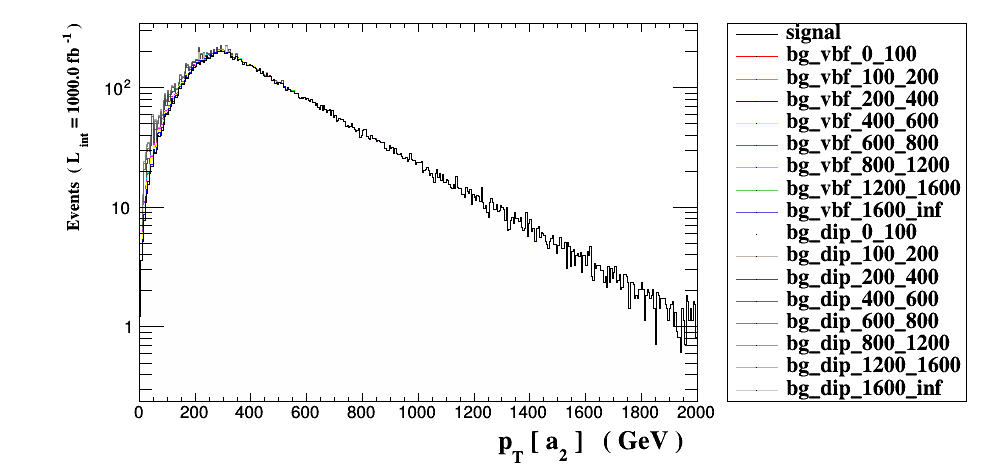
\includegraphics[scale=0.45]{selection_12.png}\\
\caption{   }
  \end{center}
\end{figure}
      \newpage
\subsection{ Histogram 14}

\textbf{* Plot: THT}\\
   \begin{table}[H]
  \begin{center}
    \begin{tabular}{|m{23.0mm}|m{23.0mm}|m{18.0mm}|m{19.0mm}|m{19.0mm}|m{19.0mm}|m{19.0mm}|}
      \hline
      {\cellcolor{yellow}         Dataset}& {\cellcolor{yellow}         Integral}& {\cellcolor{yellow}         Entries per event}& {\cellcolor{yellow}         Mean}& {\cellcolor{yellow}         RMS}& {\cellcolor{yellow}         \% underflow}& {\cellcolor{yellow}         \% overflow}\\
      \hline
      {\cellcolor{white}         signal}& {\cellcolor{white}         19174}& {\cellcolor{white}         1.0}& {\cellcolor{white}         473.074}& {\cellcolor{white}         297.8}& {\cellcolor{green}         0.0}& {\cellcolor{green}         0.0}\\
      \hline
      {\cellcolor{white}         bg\_vbf\_0\_100}& {\cellcolor{white}         1.22}& {\cellcolor{white}         1.0}& {\cellcolor{white}         74.6978}& {\cellcolor{white}         15.53}& {\cellcolor{green}         0.0}& {\cellcolor{green}         0.0}\\
      \hline
      {\cellcolor{white}         bg\_vbf\_100\_200}& {\cellcolor{white}         29.1}& {\cellcolor{white}         1.0}& {\cellcolor{white}         163.344}& {\cellcolor{white}         25.73}& {\cellcolor{green}         0.0}& {\cellcolor{green}         0.0}\\
      \hline
      {\cellcolor{white}         bg\_vbf\_200\_400}& {\cellcolor{white}         151}& {\cellcolor{white}         1.0}& {\cellcolor{white}         305.428}& {\cellcolor{white}         55.11}& {\cellcolor{green}         0.0}& {\cellcolor{green}         0.0}\\
      \hline
      {\cellcolor{white}         bg\_vbf\_400\_600}& {\cellcolor{white}         110}& {\cellcolor{white}         1.0}& {\cellcolor{white}         485.133}& {\cellcolor{white}         55.92}& {\cellcolor{green}         0.0}& {\cellcolor{green}         0.0}\\
      \hline
      {\cellcolor{white}         bg\_vbf\_600\_800}& {\cellcolor{white}         41.0}& {\cellcolor{white}         1.0}& {\cellcolor{white}         680.936}& {\cellcolor{white}         55.85}& {\cellcolor{green}         0.0}& {\cellcolor{green}         0.0}\\
      \hline
      {\cellcolor{white}         bg\_vbf\_800\_1200}& {\cellcolor{white}         15.6}& {\cellcolor{white}         1.0}& {\cellcolor{white}         929.067}& {\cellcolor{white}         102.2}& {\cellcolor{green}         0.0}& {\cellcolor{green}         0.0}\\
      \hline
      {\cellcolor{white}         bg\_vbf\_1200\_1600}& {\cellcolor{white}         1.37}& {\cellcolor{white}         1.0}& {\cellcolor{white}         1324.24}& {\cellcolor{white}         99.5}& {\cellcolor{green}         0.0}& {\cellcolor{green}         0.0}\\
      \hline
      {\cellcolor{white}         bg\_vbf\_1600\_inf}& {\cellcolor{white}         0.145}& {\cellcolor{white}         1.0}& {\cellcolor{white}         1789.2}& {\cellcolor{white}         191.2}& {\cellcolor{green}         0.0}& {\cellcolor{green}         0.0}\\
      \hline
      {\cellcolor{white}         bg\_dip\_0\_100}& {\cellcolor{white}         0.0 +/\-- 0.0}& {\cellcolor{white}         0.}& {\cellcolor{white}         0.0}& {\cellcolor{white}         0.0}& {\cellcolor{green}         0.0}& {\cellcolor{green}         0.0}\\
      \hline
      {\cellcolor{white}         bg\_dip\_100\_200}& {\cellcolor{white}         79.0}& {\cellcolor{white}         1.0}& {\cellcolor{white}         148.168}& {\cellcolor{white}         37.58}& {\cellcolor{green}         0.0}& {\cellcolor{green}         0.0}\\
      \hline
      {\cellcolor{white}         bg\_dip\_200\_400}& {\cellcolor{white}         477}& {\cellcolor{white}         1.0}& {\cellcolor{white}         312.487}& {\cellcolor{white}         53.59}& {\cellcolor{green}         0.0}& {\cellcolor{green}         0.0}\\
      \hline
      {\cellcolor{white}         bg\_dip\_400\_600}& {\cellcolor{white}         306}& {\cellcolor{white}         1.0}& {\cellcolor{white}         483.667}& {\cellcolor{white}         56.67}& {\cellcolor{green}         0.0}& {\cellcolor{green}         0.0}\\
      \hline
      {\cellcolor{white}         bg\_dip\_600\_800}& {\cellcolor{white}         90.0}& {\cellcolor{white}         1.0}& {\cellcolor{white}         677.891}& {\cellcolor{white}         53.6}& {\cellcolor{green}         0.0}& {\cellcolor{green}         0.0}\\
      \hline
      {\cellcolor{white}         bg\_dip\_800\_1200}& {\cellcolor{white}         36.8}& {\cellcolor{white}         1.0}& {\cellcolor{white}         924.952}& {\cellcolor{white}         102.7}& {\cellcolor{green}         0.0}& {\cellcolor{green}         0.0}\\
      \hline
      {\cellcolor{white}         bg\_dip\_1200\_1600}& {\cellcolor{white}         2.63}& {\cellcolor{white}         1.0}& {\cellcolor{white}         1350.6}& {\cellcolor{white}         122.7}& {\cellcolor{green}         0.0}& {\cellcolor{green}         0.0}\\
      \hline
      {\cellcolor{white}         bg\_dip\_1600\_inf}& {\cellcolor{white}         0.244}& {\cellcolor{white}         1.0}& {\cellcolor{white}         1813.83}& {\cellcolor{white}         223.3}& {\cellcolor{green}         0.0}& {\cellcolor{green}         0.0}\\
\hline
    \end{tabular}
  \end{center}
\end{table}

\begin{figure}[H]
  \begin{center}
    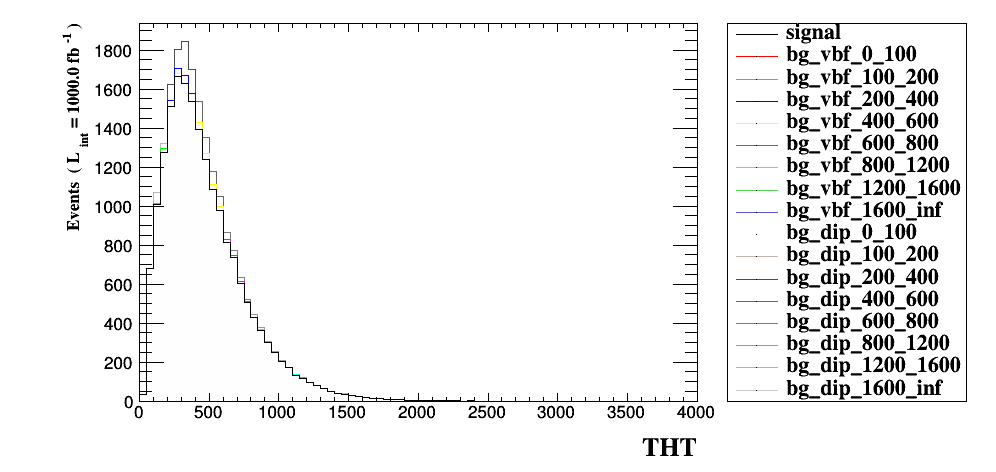
\includegraphics[scale=0.45]{selection_13.png}\\
\caption{   }
  \end{center}
\end{figure}
      \newpage
\subsection{ Histogram 15}

\textbf{* Plot: MET}\\
   \begin{table}[H]
  \begin{center}
    \begin{tabular}{|m{23.0mm}|m{23.0mm}|m{18.0mm}|m{19.0mm}|m{19.0mm}|m{19.0mm}|m{19.0mm}|}
      \hline
      {\cellcolor{yellow}         Dataset}& {\cellcolor{yellow}         Integral}& {\cellcolor{yellow}         Entries per event}& {\cellcolor{yellow}         Mean}& {\cellcolor{yellow}         RMS}& {\cellcolor{yellow}         \% underflow}& {\cellcolor{yellow}         \% overflow}\\
      \hline
      {\cellcolor{white}         signal}& {\cellcolor{white}         19174}& {\cellcolor{white}         1.0}& {\cellcolor{white}         9.23621e-09}& {\cellcolor{white}         1.193e-08}& {\cellcolor{green}         0.0}& {\cellcolor{green}         0.0}\\
      \hline
      {\cellcolor{white}         bg\_vbf\_0\_100}& {\cellcolor{white}         1.22}& {\cellcolor{white}         1.0}& {\cellcolor{white}         2.92664e-09}& {\cellcolor{white}         2.061e-09}& {\cellcolor{green}         0.0}& {\cellcolor{green}         0.0}\\
      \hline
      {\cellcolor{white}         bg\_vbf\_100\_200}& {\cellcolor{white}         29.1}& {\cellcolor{white}         1.0}& {\cellcolor{white}         4.59216e-09}& {\cellcolor{white}         2.634e-09}& {\cellcolor{green}         0.0}& {\cellcolor{green}         0.0}\\
      \hline
      {\cellcolor{white}         bg\_vbf\_200\_400}& {\cellcolor{white}         151}& {\cellcolor{white}         1.0}& {\cellcolor{white}         5.28184e-09}& {\cellcolor{white}         3.059e-09}& {\cellcolor{green}         0.0}& {\cellcolor{green}         0.0}\\
      \hline
      {\cellcolor{white}         bg\_vbf\_400\_600}& {\cellcolor{white}         110}& {\cellcolor{white}         1.0}& {\cellcolor{white}         5.56314e-09}& {\cellcolor{white}         3.759e-09}& {\cellcolor{green}         0.0}& {\cellcolor{green}         0.0}\\
      \hline
      {\cellcolor{white}         bg\_vbf\_600\_800}& {\cellcolor{white}         41.0}& {\cellcolor{white}         1.0}& {\cellcolor{white}         5.7028e-09}& {\cellcolor{white}         3.425e-09}& {\cellcolor{green}         0.0}& {\cellcolor{green}         0.0}\\
      \hline
      {\cellcolor{white}         bg\_vbf\_800\_1200}& {\cellcolor{white}         15.6}& {\cellcolor{white}         1.0}& {\cellcolor{white}         6.73764e-09}& {\cellcolor{white}         5.92e-09}& {\cellcolor{green}         0.0}& {\cellcolor{green}         0.0}\\
      \hline
      {\cellcolor{white}         bg\_vbf\_1200\_1600}& {\cellcolor{white}         1.37}& {\cellcolor{white}         1.0}& {\cellcolor{white}         1.72505e-08}& {\cellcolor{white}         1.831e-08}& {\cellcolor{green}         0.0}& {\cellcolor{green}         0.0}\\
      \hline
      {\cellcolor{white}         bg\_vbf\_1600\_inf}& {\cellcolor{white}         0.145}& {\cellcolor{white}         1.0}& {\cellcolor{white}         3.09154e-08}& {\cellcolor{white}         2.364e-08}& {\cellcolor{green}         0.0}& {\cellcolor{green}         0.0}\\
      \hline
      {\cellcolor{white}         bg\_dip\_0\_100}& {\cellcolor{white}         0.0 +/\-- 0.0}& {\cellcolor{white}         0.}& {\cellcolor{white}         0.0}& {\cellcolor{white}         0.0}& {\cellcolor{green}         0.0}& {\cellcolor{green}         0.0}\\
      \hline
      {\cellcolor{white}         bg\_dip\_100\_200}& {\cellcolor{white}         79.0}& {\cellcolor{white}         1.0}& {\cellcolor{white}         2.6048e-09}& {\cellcolor{white}         5.584e-10}& {\cellcolor{green}         0.0}& {\cellcolor{green}         0.0}\\
      \hline
      {\cellcolor{white}         bg\_dip\_200\_400}& {\cellcolor{white}         477}& {\cellcolor{white}         1.0}& {\cellcolor{white}         5.15652e-09}& {\cellcolor{white}         2.886e-09}& {\cellcolor{green}         0.0}& {\cellcolor{green}         0.0}\\
      \hline
      {\cellcolor{white}         bg\_dip\_400\_600}& {\cellcolor{white}         306}& {\cellcolor{white}         1.0}& {\cellcolor{white}         5.26293e-09}& {\cellcolor{white}         2.848e-09}& {\cellcolor{green}         0.0}& {\cellcolor{green}         0.0}\\
      \hline
      {\cellcolor{white}         bg\_dip\_600\_800}& {\cellcolor{white}         90.0}& {\cellcolor{white}         1.0}& {\cellcolor{white}         5.42862e-09}& {\cellcolor{white}         2.905e-09}& {\cellcolor{green}         0.0}& {\cellcolor{green}         0.0}\\
      \hline
      {\cellcolor{white}         bg\_dip\_800\_1200}& {\cellcolor{white}         36.8}& {\cellcolor{white}         1.0}& {\cellcolor{white}         7.13192e-09}& {\cellcolor{white}         8.331e-09}& {\cellcolor{green}         0.0}& {\cellcolor{green}         0.0}\\
      \hline
      {\cellcolor{white}         bg\_dip\_1200\_1600}& {\cellcolor{white}         2.63}& {\cellcolor{white}         1.0}& {\cellcolor{white}         2.55869e-08}& {\cellcolor{white}         2.401e-08}& {\cellcolor{green}         0.0}& {\cellcolor{green}         0.0}\\
      \hline
      {\cellcolor{white}         bg\_dip\_1600\_inf}& {\cellcolor{white}         0.244}& {\cellcolor{white}         1.0}& {\cellcolor{white}         3.47198e-08}& {\cellcolor{white}         2.306e-08}& {\cellcolor{green}         0.0}& {\cellcolor{green}         0.0}\\
\hline
    \end{tabular}
  \end{center}
\end{table}

\begin{figure}[H]
  \begin{center}
    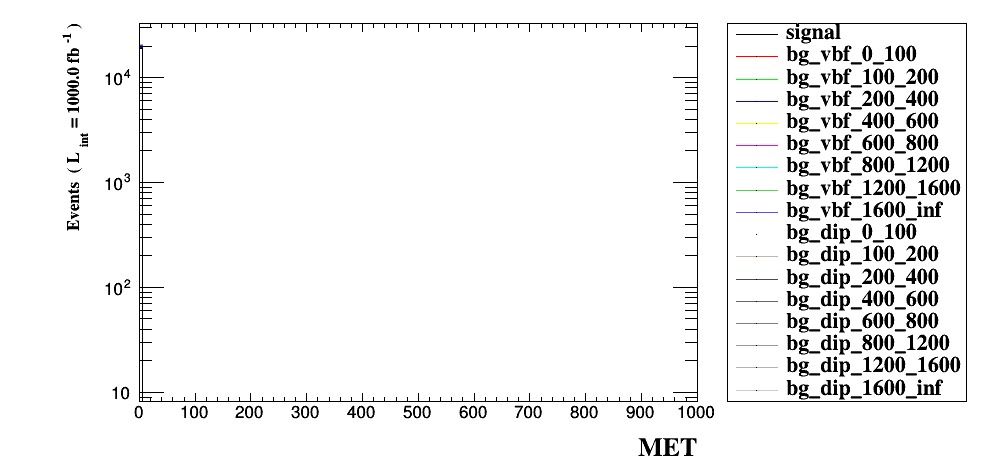
\includegraphics[scale=0.45]{selection_14.png}\\
\caption{   }
  \end{center}
\end{figure}
      \newpage
\subsection{ Histogram 16}

\textbf{* Plot: TET}\\
   \begin{table}[H]
  \begin{center}
    \begin{tabular}{|m{23.0mm}|m{23.0mm}|m{18.0mm}|m{19.0mm}|m{19.0mm}|m{19.0mm}|m{19.0mm}|}
      \hline
      {\cellcolor{yellow}         Dataset}& {\cellcolor{yellow}         Integral}& {\cellcolor{yellow}         Entries per event}& {\cellcolor{yellow}         Mean}& {\cellcolor{yellow}         RMS}& {\cellcolor{yellow}         \% underflow}& {\cellcolor{yellow}         \% overflow}\\
      \hline
      {\cellcolor{white}         signal}& {\cellcolor{white}         19174}& {\cellcolor{white}         1.0}& {\cellcolor{white}         1678.89}& {\cellcolor{white}         734.6}& {\cellcolor{green}         0.0}& {\cellcolor{green}         0.0}\\
      \hline
      {\cellcolor{white}         bg\_vbf\_0\_100}& {\cellcolor{white}         1.22}& {\cellcolor{white}         1.0}& {\cellcolor{white}         814.434}& {\cellcolor{white}         141.3}& {\cellcolor{green}         0.0}& {\cellcolor{green}         0.0}\\
      \hline
      {\cellcolor{white}         bg\_vbf\_100\_200}& {\cellcolor{white}         29.1}& {\cellcolor{white}         1.0}& {\cellcolor{white}         822.463}& {\cellcolor{white}         164.7}& {\cellcolor{green}         0.0}& {\cellcolor{green}         0.0}\\
      \hline
      {\cellcolor{white}         bg\_vbf\_200\_400}& {\cellcolor{white}         151}& {\cellcolor{white}         1.0}& {\cellcolor{white}         906.139}& {\cellcolor{white}         195.9}& {\cellcolor{green}         0.0}& {\cellcolor{green}         0.0}\\
      \hline
      {\cellcolor{white}         bg\_vbf\_400\_600}& {\cellcolor{white}         110}& {\cellcolor{white}         1.0}& {\cellcolor{white}         1080.57}& {\cellcolor{white}         211.3}& {\cellcolor{green}         0.0}& {\cellcolor{green}         0.0}\\
      \hline
      {\cellcolor{white}         bg\_vbf\_600\_800}& {\cellcolor{white}         41.0}& {\cellcolor{white}         1.0}& {\cellcolor{white}         1355.11}& {\cellcolor{white}         216.7}& {\cellcolor{green}         0.0}& {\cellcolor{green}         0.0}\\
      \hline
      {\cellcolor{white}         bg\_vbf\_800\_1200}& {\cellcolor{white}         15.6}& {\cellcolor{white}         1.0}& {\cellcolor{white}         1745.89}& {\cellcolor{white}         291.5}& {\cellcolor{green}         0.0}& {\cellcolor{green}         0.0}\\
      \hline
      {\cellcolor{white}         bg\_vbf\_1200\_1600}& {\cellcolor{white}         1.37}& {\cellcolor{white}         1.0}& {\cellcolor{white}         2382.74}& {\cellcolor{white}         401.9}& {\cellcolor{green}         0.0}& {\cellcolor{green}         0.0}\\
      \hline
      {\cellcolor{white}         bg\_vbf\_1600\_inf}& {\cellcolor{white}         0.145}& {\cellcolor{white}         1.0}& {\cellcolor{white}         3296.68}& {\cellcolor{white}         649.6}& {\cellcolor{green}         0.0}& {\cellcolor{green}         0.0}\\
      \hline
      {\cellcolor{white}         bg\_dip\_0\_100}& {\cellcolor{white}         0.0 +/\-- 0.0}& {\cellcolor{white}         0.}& {\cellcolor{white}         0.0}& {\cellcolor{white}         0.0}& {\cellcolor{green}         0.0}& {\cellcolor{green}         0.0}\\
      \hline
      {\cellcolor{white}         bg\_dip\_100\_200}& {\cellcolor{white}         79.0}& {\cellcolor{white}         1.0}& {\cellcolor{white}         728.733}& {\cellcolor{white}         80.65}& {\cellcolor{green}         0.0}& {\cellcolor{green}         0.0}\\
      \hline
      {\cellcolor{white}         bg\_dip\_200\_400}& {\cellcolor{white}         477}& {\cellcolor{white}         1.0}& {\cellcolor{white}         892.065}& {\cellcolor{white}         159.2}& {\cellcolor{green}         0.0}& {\cellcolor{green}         0.0}\\
      \hline
      {\cellcolor{white}         bg\_dip\_400\_600}& {\cellcolor{white}         306}& {\cellcolor{white}         1.0}& {\cellcolor{white}         1103.5}& {\cellcolor{white}         208.7}& {\cellcolor{green}         0.0}& {\cellcolor{green}         0.0}\\
      \hline
      {\cellcolor{white}         bg\_dip\_600\_800}& {\cellcolor{white}         90.0}& {\cellcolor{white}         1.0}& {\cellcolor{white}         1421.58}& {\cellcolor{white}         241.6}& {\cellcolor{green}         0.0}& {\cellcolor{green}         0.0}\\
      \hline
      {\cellcolor{white}         bg\_dip\_800\_1200}& {\cellcolor{white}         36.8}& {\cellcolor{white}         1.0}& {\cellcolor{white}         1833.63}& {\cellcolor{white}         311.4}& {\cellcolor{green}         0.0}& {\cellcolor{green}         0.0}\\
      \hline
      {\cellcolor{white}         bg\_dip\_1200\_1600}& {\cellcolor{white}         2.63}& {\cellcolor{white}         1.0}& {\cellcolor{white}         2597.16}& {\cellcolor{white}         496.1}& {\cellcolor{green}         0.0}& {\cellcolor{green}         0.0}\\
      \hline
      {\cellcolor{white}         bg\_dip\_1600\_inf}& {\cellcolor{white}         0.244}& {\cellcolor{white}         1.0}& {\cellcolor{white}         3541.73}& {\cellcolor{white}         662.3}& {\cellcolor{green}         0.0}& {\cellcolor{green}         0.0}\\
\hline
    \end{tabular}
  \end{center}
\end{table}

\begin{figure}[H]
  \begin{center}
    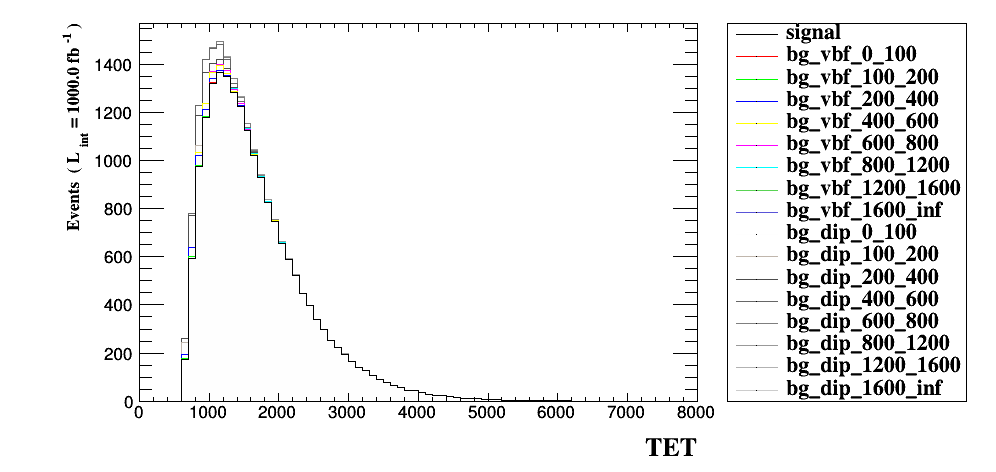
\includegraphics[scale=0.45]{selection_15.png}\\
\caption{   }
  \end{center}
\end{figure}
      % -----------------------------------------------------------------------------
%                                SECTION Summary                                
% -----------------------------------------------------------------------------
\newpage
\section{ Summary}

\subsection{Cut-flow charts}

\begin{itemize}
  \item How to compare signal (S) and background (B): \textcolor{blue}{S/\-sqrt(S+B+(xB)**2)} .
   \item Object definition selections are indicated in cyan.  \item Reject and select are indicated by 'REJ' and 'SEL' respectively
\end{itemize}
\begin{table}[H]
  \begin{center}
    \begin{tabular}{|m{36.0mm}|m{36.0mm}|m{36.0mm}|m{33.0mm}|}
      \hline
      {\cellcolor{yellow}        Cuts}& {\cellcolor{yellow}         Signal (S)}& {\cellcolor{yellow}         Background (B)}& {\cellcolor{yellow}         S vs B}\\
      \hline
      {\cellcolor{white}         Initial (no cut)}& {\cellcolor{white}         102352.1 +/\-- 28.2}& {\cellcolor{white}         102837909 +/\-- 121936}& {\cellcolor{white}         10.08798 +/\-- 0.00659}\\
      \hline
      {\cellcolor{white} SEL: ( ( sdETA ( jets[1] jets[2] ) > 3.6 or sdETA }& {\cellcolor{white}         19174 +/\-- 124}& {\cellcolor{white}         1343.7 +/\-- 36.7}& {\cellcolor{white}         133.86 +/\-- 0.48}\\
\hline
    \end{tabular}
  \end{center}
\end{table}

\end{document}
